\documentclass{article}
\usepackage[left=2cm,right=2cm,top=2cm,bottom=4cm,bindingoffset=0cm]{geometry}

\usepackage[utf8]{inputenc}
\usepackage[russian]{babel}
\usepackage{graphicx}
\usepackage{amsmath}
\usepackage{breqn}
\usepackage{wrapfig}
\usepackage{float}
\usepackage{multirow}
\usepackage{caption}
\usepackage{subcaption}

\graphicspath{ {./data/images} }
\author{Александр Романов Б01-107}
\date{}
\title{18 Пассивные электрические цепи}

\begin{document}
\maketitle


\section{Задание 1}
\subsection{low-pass filter}
Соберём интегрирующую цепь (low-pass filter) и проведём измерения.

\begin{figure}[H]
    \centering
    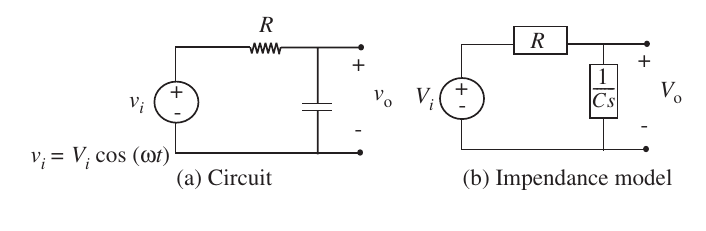
\includegraphics[width=0.8\textwidth]{low-pass-filter.png}
    \caption{low-pass filter}
\end{figure}

\[C = 1\;\mu F,\; R = 100\;\Omega,\; f_0 = 1.6\;kHz\]
\begin{table}[H]
    \centering
    \begin{tabular}{|c|c|}
        \hline
    \(\log_2\left(\frac{f}{f_0}\right)\)&\(20\ln(K)\)\\\hline
    -2 & -0.76  \\\hline
    -1 & -1.57  \\\hline
    0  & -6.20  \\\hline
    1  & -13.26 \\\hline
    2  & -22.63 \\\hline
    3  & -35.84 \\\hline
    \end{tabular}
\end{table}

\begin{figure}[H]
    \centering
    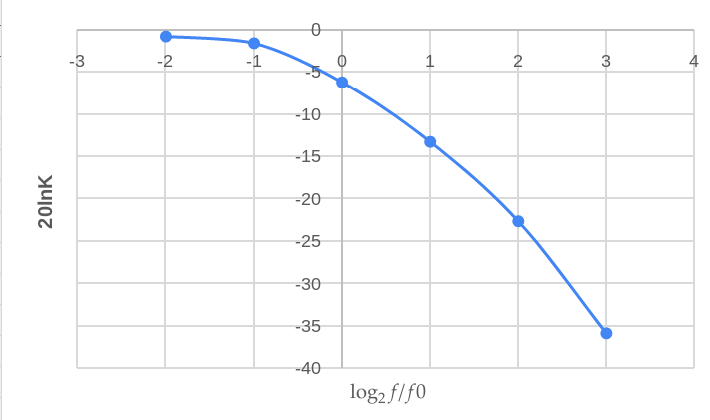
\includegraphics[width=0.8\textwidth]{18.1.png}
    \caption{Frequency response of low-pass filter }
\end{figure}

Подключим генератор прямоугольных импульсов и по осциллограмме переходной характеристики
оценим постоянную времени \(\tau\):
\[\tau = 78\;\mu s\]
\[f_0 = \frac{1}{2\pi\tau}\simeq 2\; kHz\]
Что близко к \(f_0\) полученному в начале.
\subsection{hight-pass filter}
Превратим интегрирующую цепь в дифференцирующую и проведём аналогичные измерения.
\[C = 1\;\mu F,\; R = 100\;\Omega,\; f_0 = 1.6\;kHz\]

\begin{table}[H]
    \centering
    \begin{tabular}{|c|c|}
    \hline
    \(\log_2\left(\frac{f}{f_0}\right)\)&\(20\ln(K)\)\\\hline
    -2 & -30.84 \\\hline
    -1 & -17.75 \\\hline
    0  & -9.35  \\\hline
    1  & -3.34  \\\hline
    2  & -1.33  \\\hline
    3  & -0.34  \\\hline
    \end{tabular}
\end{table}

\begin{figure}[H]
    \centering
    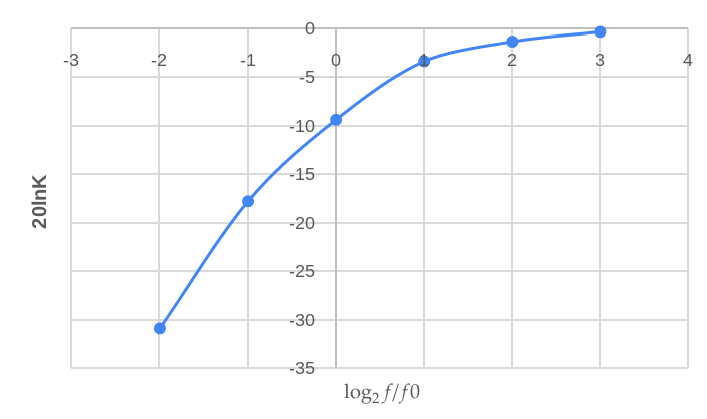
\includegraphics[width=0.8\textwidth]{18.2.png}
    \caption{Frequency response of hight-pass filter }
\end{figure}

Подключим генератор прямоугольных импульсов и по осциллограмме переходной характеристики
оценим постоянную времени \(\tau\):
\[\tau = 144\;\mu s\]
\[f_0 = \frac{1}{2\pi\tau}\simeq 1\; kHz\]


\subsection{rcint.cir}
Откроем в MicroCap модель \textbf{rcint.cir}. Изучим графики частотной и фазовой характеристики.

\begin{figure}[H]
\centering
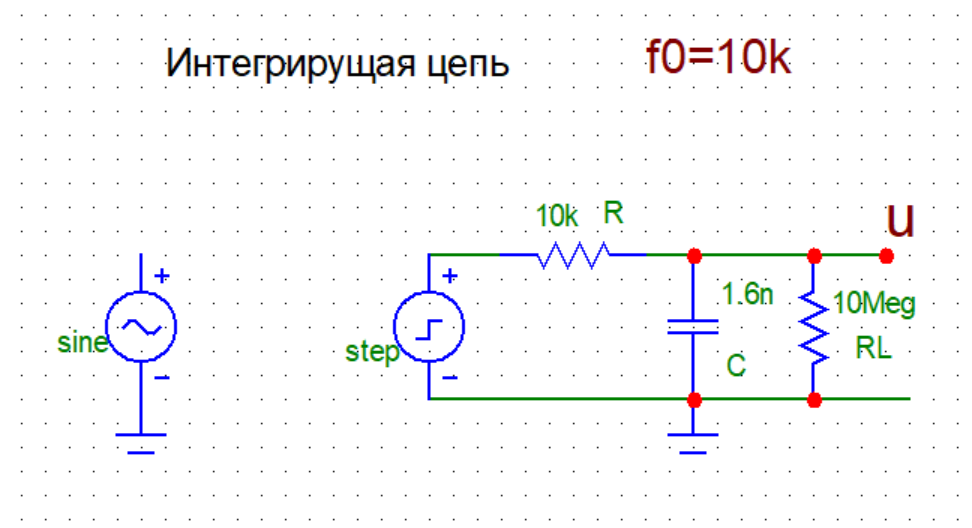
\includegraphics[scale=0.4]{rcint_img.png}
\label{fig:Image1}
\end{figure}

\begin{figure}[H]
\centering
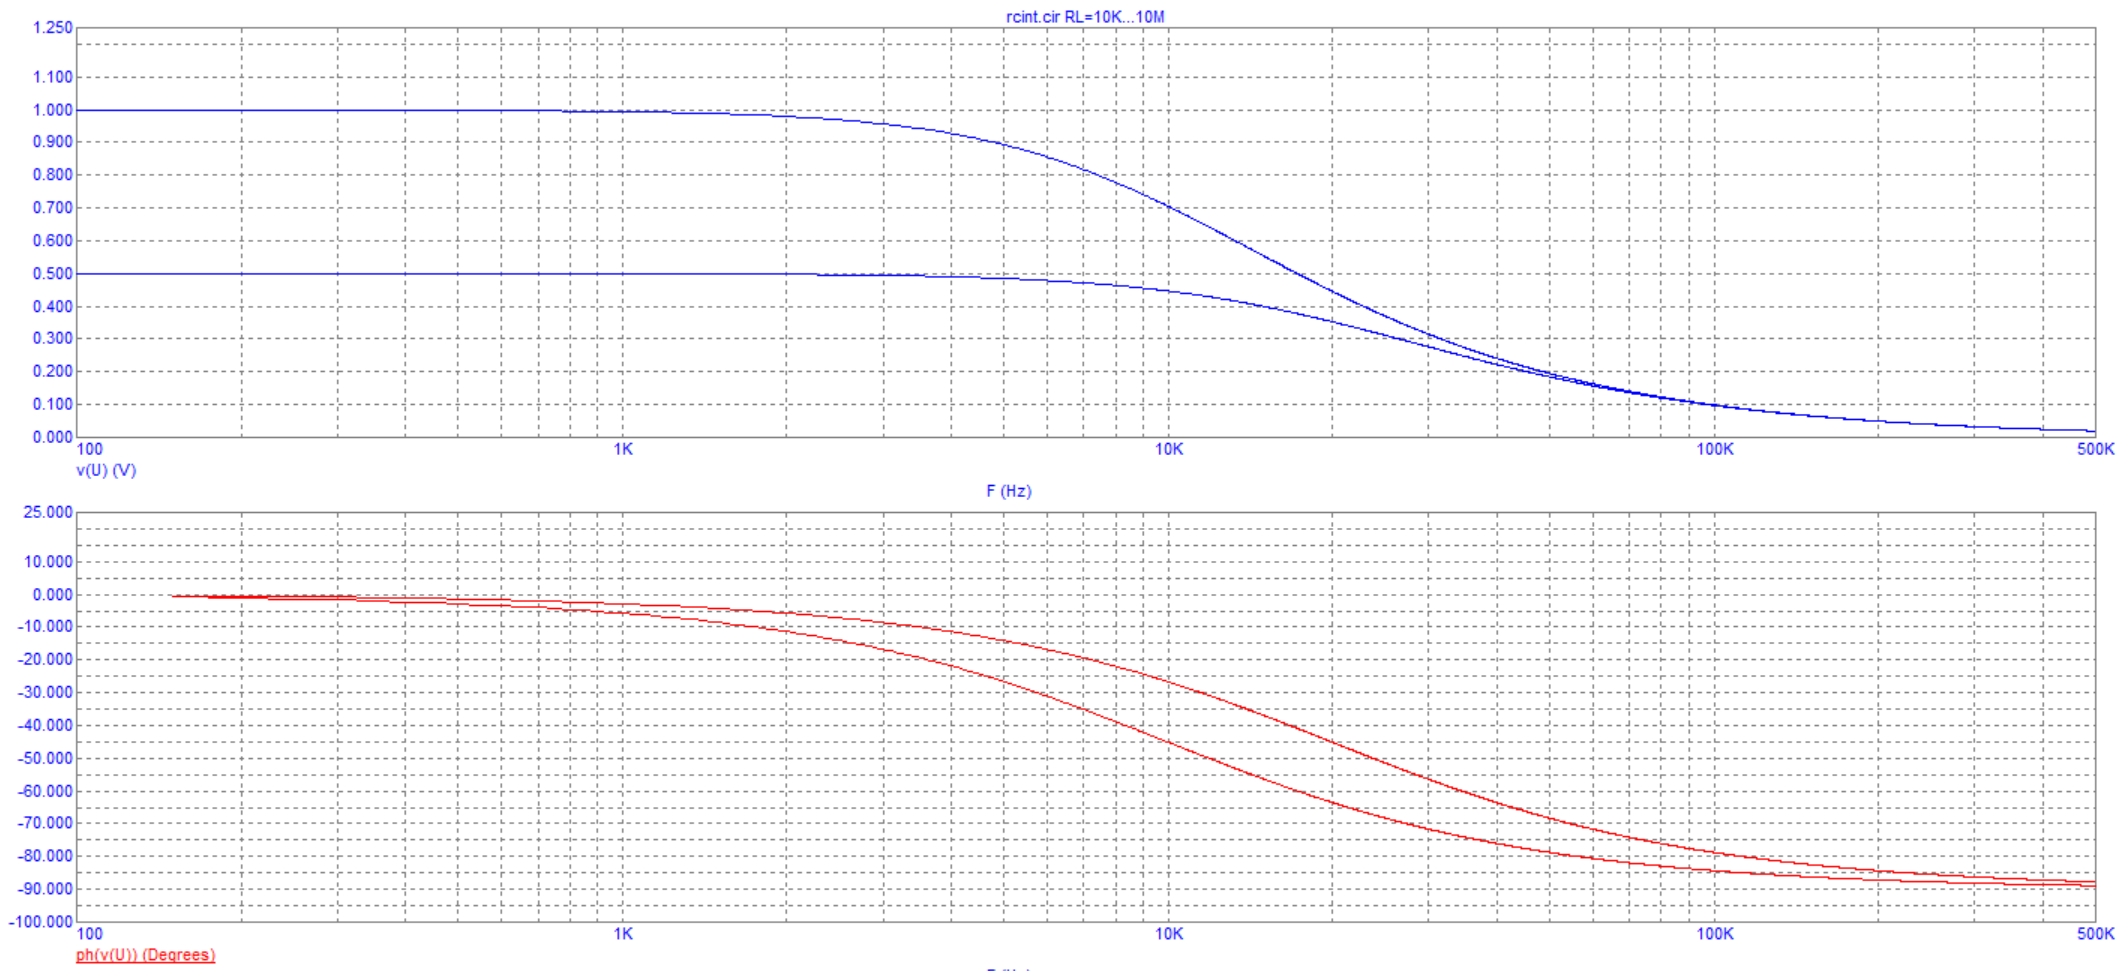
\includegraphics[scale=0.4]{rcint_AC.png}
\label{fig:Image1}
\end{figure}

По графику видно, что передаточная функция цепи принимает вид:

\[H(p) = \frac{K_0}{1 + p\tau}; \quad K_0 = \frac{R_L}{R + R_L},\tau = (R\Vert R_L) C.\]

По графику оценим верхнюю частоту:

\[R_L = 10 \: k\Omega, \quad f_0 \simeq 10 \: kHz\]
\[R_L = 10 \: M\Omega, \quad f_0 \simeq 19,9 \: kHz\]

Изучим переходную характеристику. По графику оценим постоянную времени:

\begin{figure}[H]
\centering
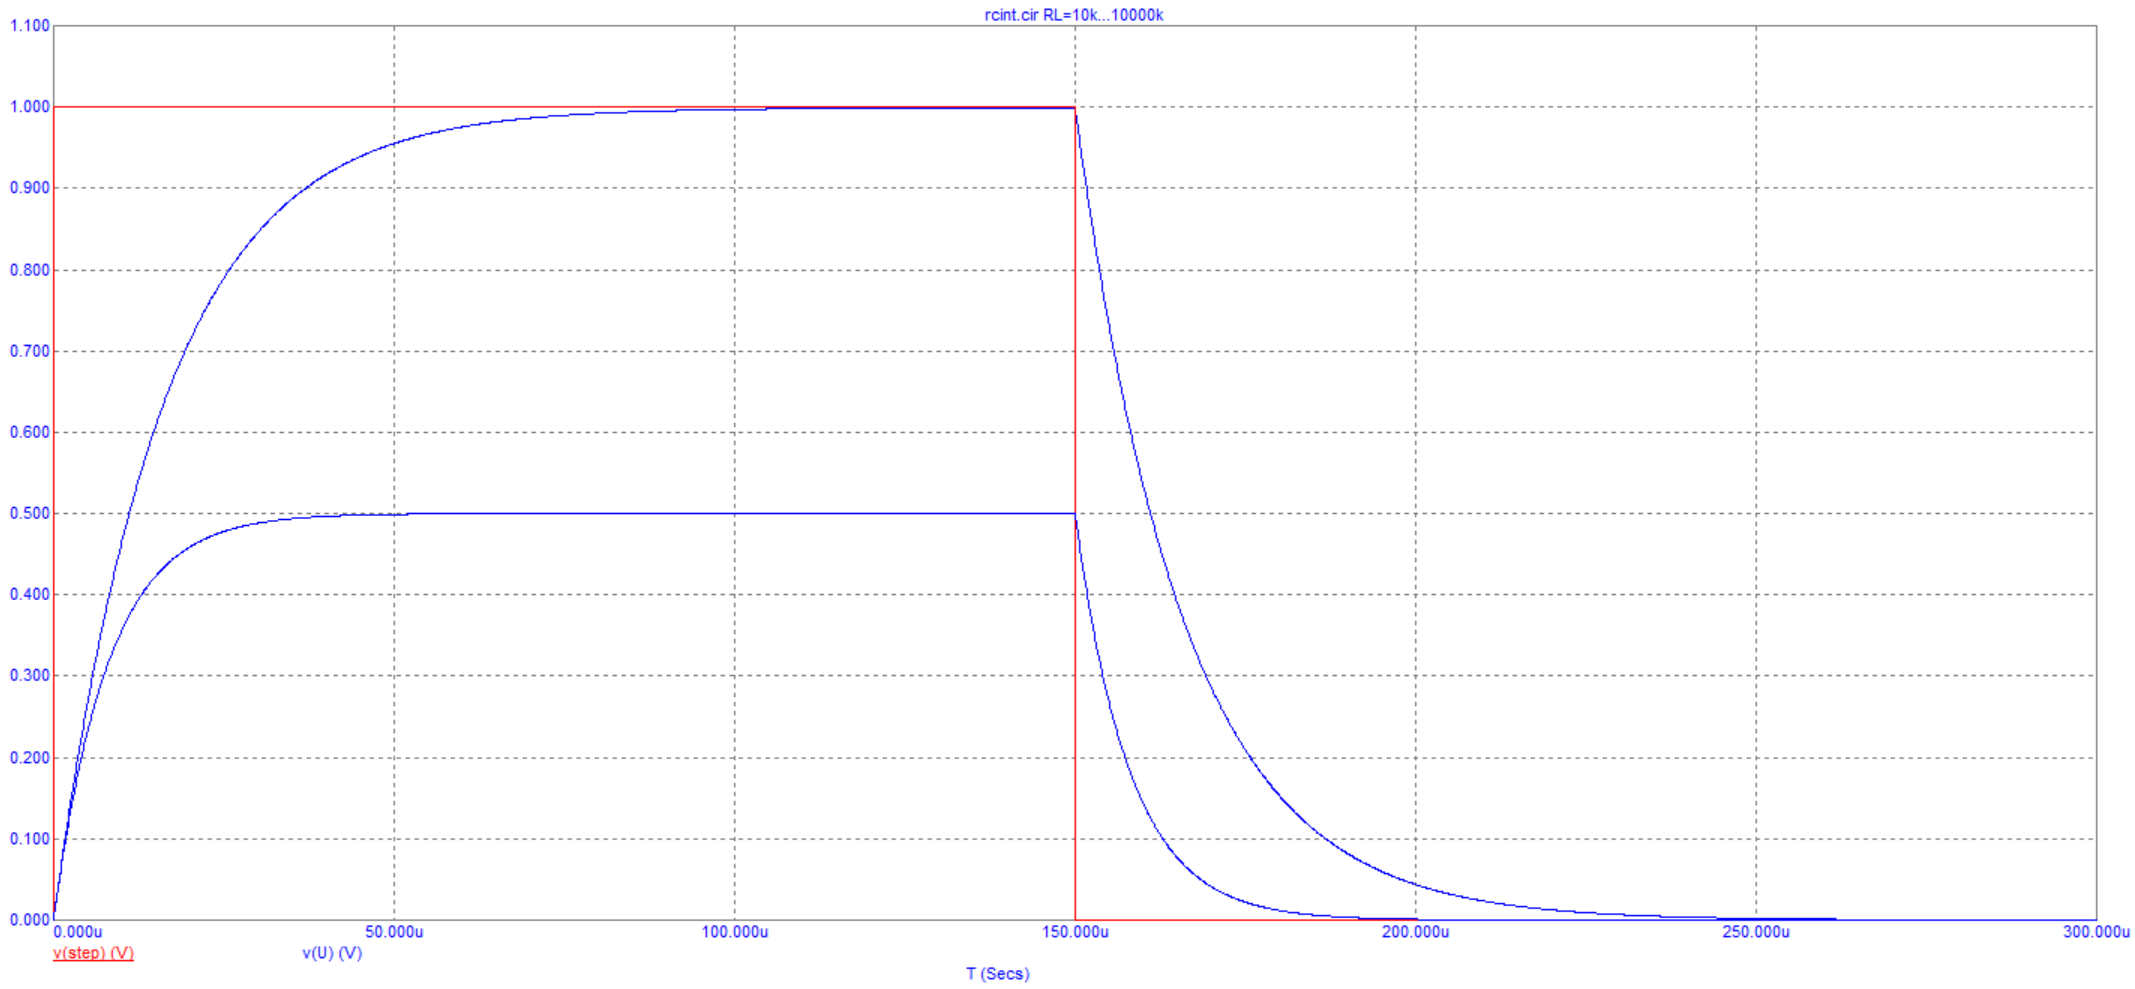
\includegraphics[scale=0.4]{rcint_Transient.png}
\label{fig:Image1}
\end{figure}

\[R_L = 10 \: k\Omega, \quad \tau \simeq 9,7 \: \mu s\]
\[R_L = 10 \: M\Omega, \quad \tau \simeq 19,6 \: \mu s\]

\subsection{rcdiff.cir}
Откроем модель \textbf{rcdiff.cir}. Изучим ее частотную и фазовую характеристики.

\begin{figure}[H]
\centering
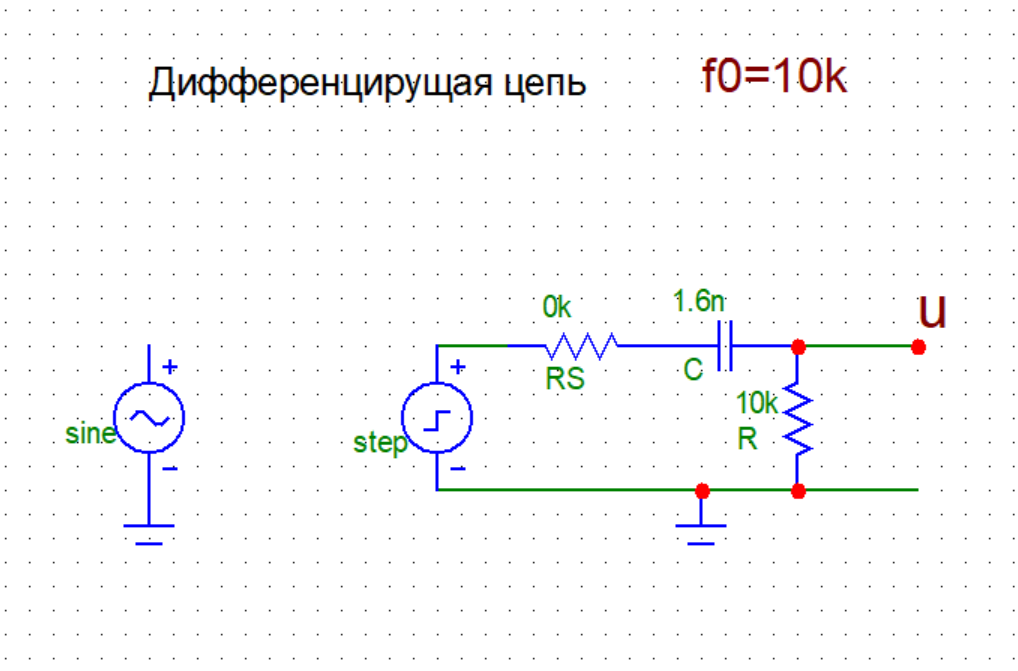
\includegraphics[scale=0.4]{rcdiff_img.png}
\label{fig:Image1}
\end{figure}

\begin{figure}[H]
\centering
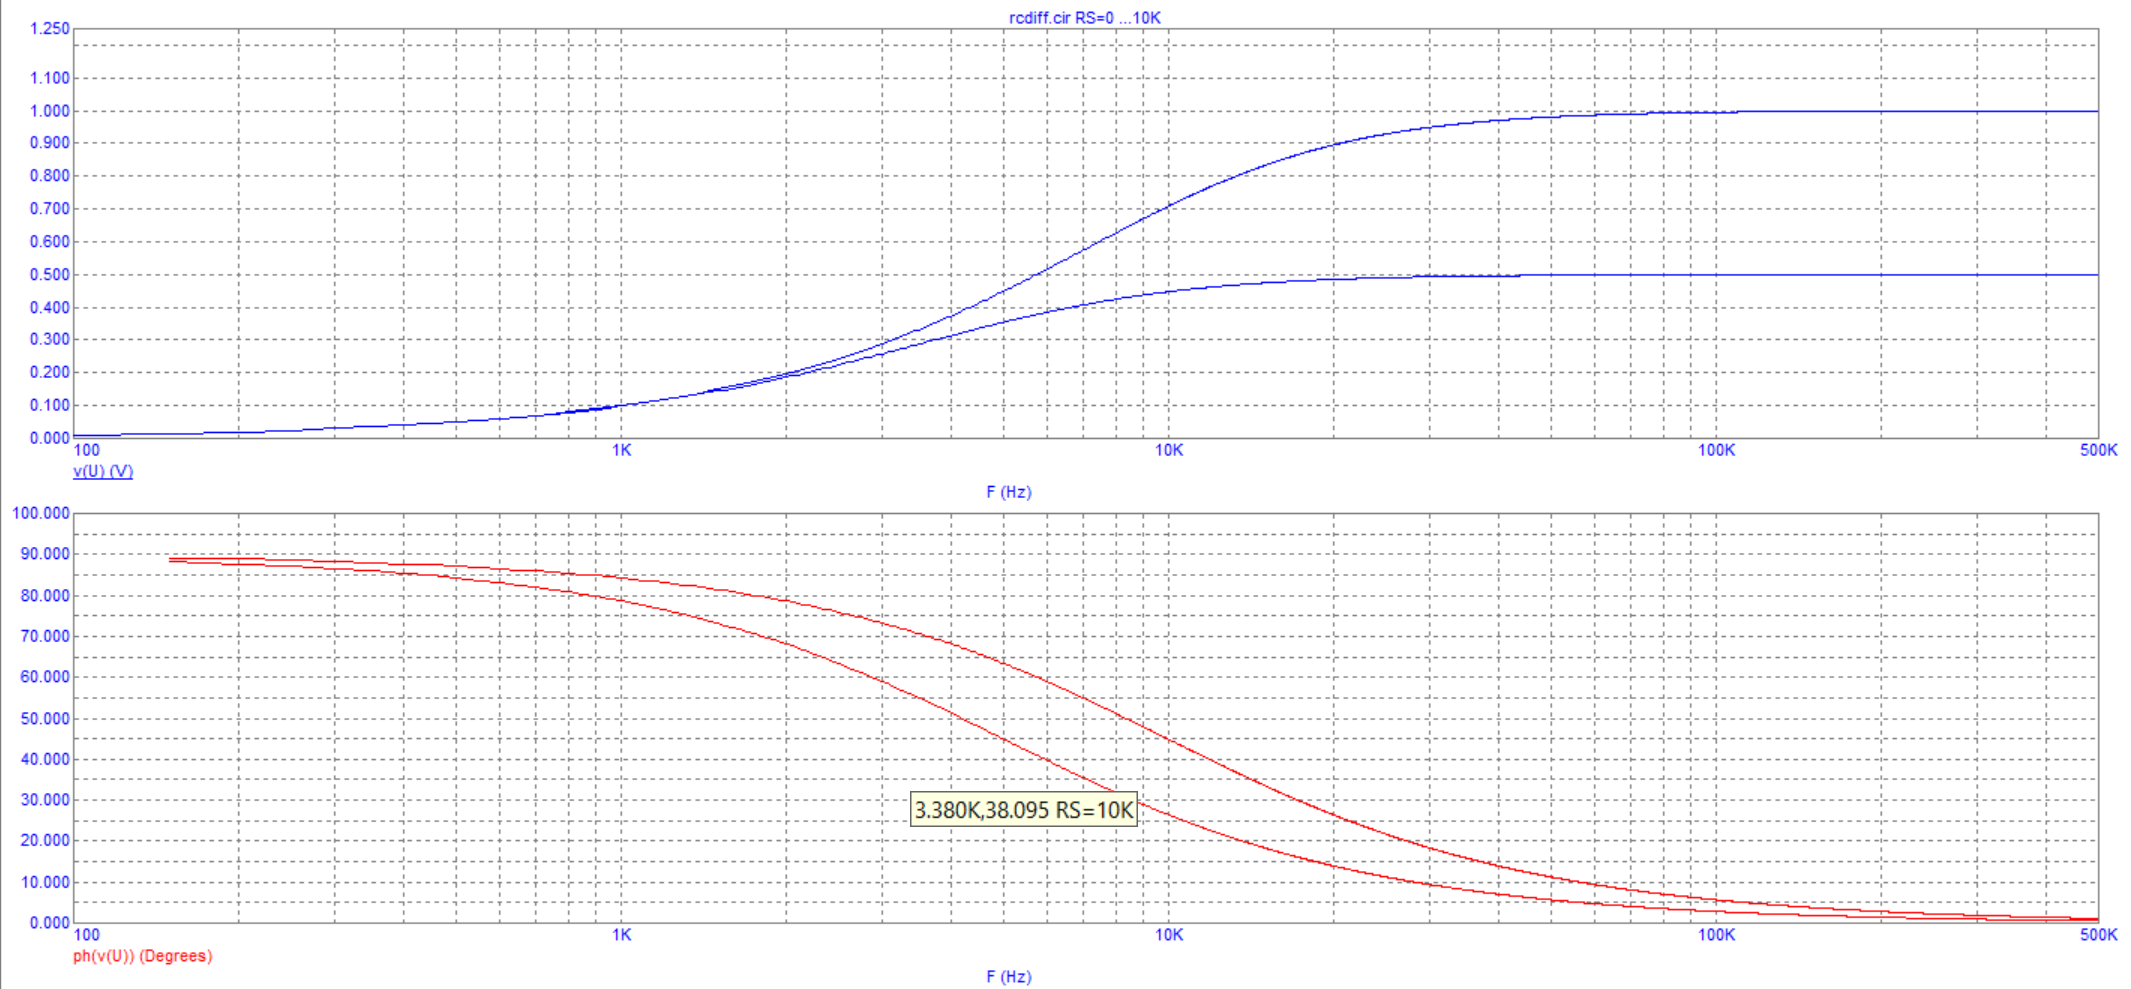
\includegraphics[scale=0.4]{rcdiff_AC.png}
\label{fig:Image1}
\end{figure}

По графику видно, что передаточная функция цепи при $R_S \neq 0$ принимает вид:

\[H(p) = \frac{K_0p\tau}{1 + p\tau}; \quad K_0 = \frac{R}{R + R_S},\tau = (R + R_S) C.\]

По графику оценим верхнюю частоту:

\[R_S = 0 \quad f_0 \simeq 9,75 \: kHz\]
\[R_S = 10 \: kHz, \quad f_0 \simeq 4,88 \: kHz\]

Изучим переходную характеристику. По графику оценим постоянную времени:

\begin{figure}[H]
\centering
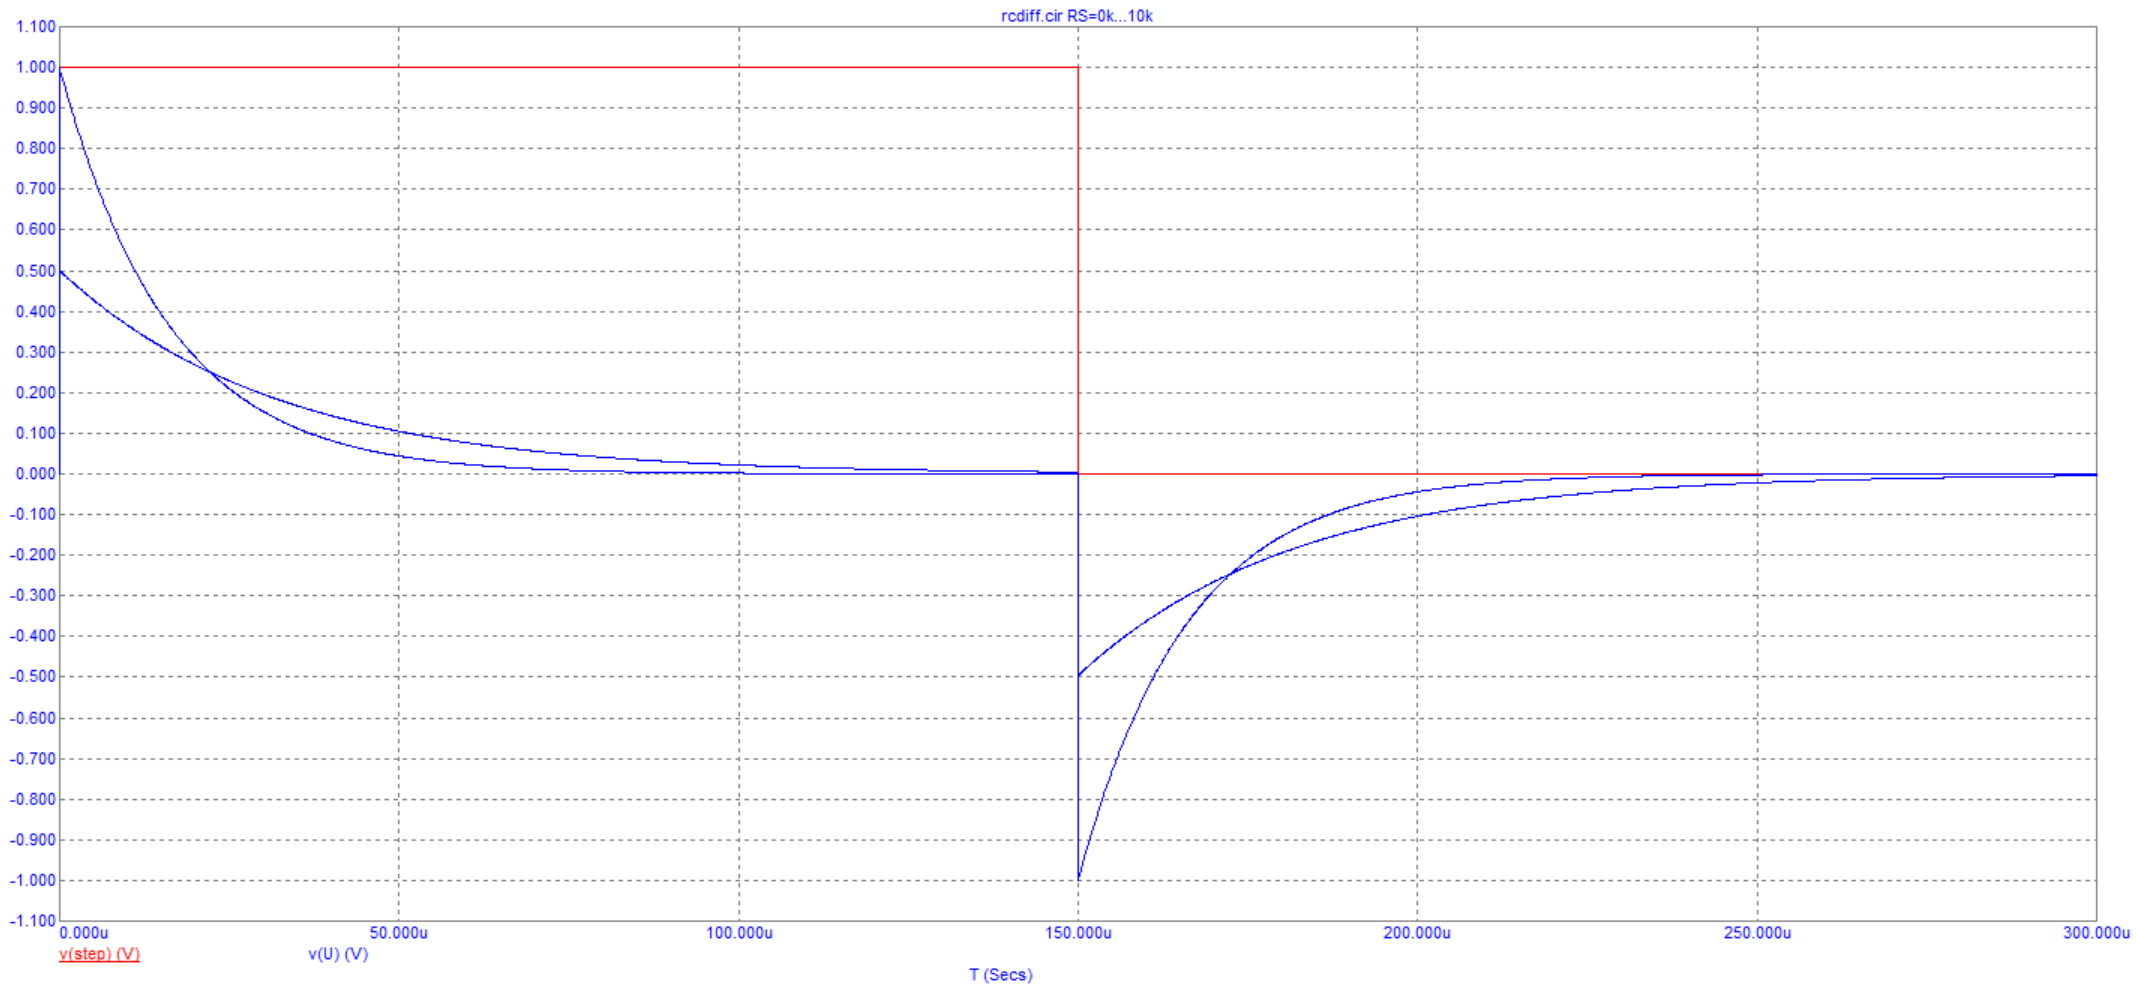
\includegraphics[scale=0.4]{rcdiff_Transient.png}
\label{fig:Image1}
\end{figure}

\[R_S = 0, \quad \tau \simeq 16,7 \: \mu s\]
\[R_S = 10 \: k\Omega, \quad \tau \simeq 31,8 \: \mu s\]

\subsection{rcpower.cir}
Откроем модель \textbf{rcpower.cir}. Изучим графики частотной зависимости потребляемых интегрирующей цепью активных и реактивных мощностей и графики мощностей на её комопонентах.

\begin{figure}[H]
\centering
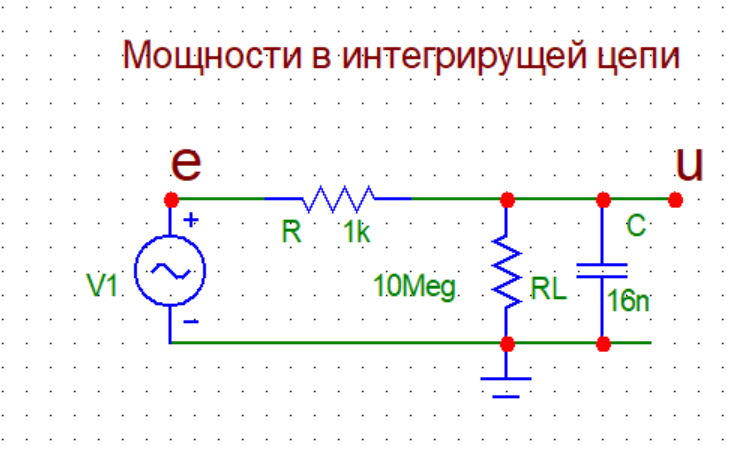
\includegraphics[scale=0.4]{rcpower_img.png}
\label{fig:Image1}
\end{figure}

\begin{figure}[H]
\centering
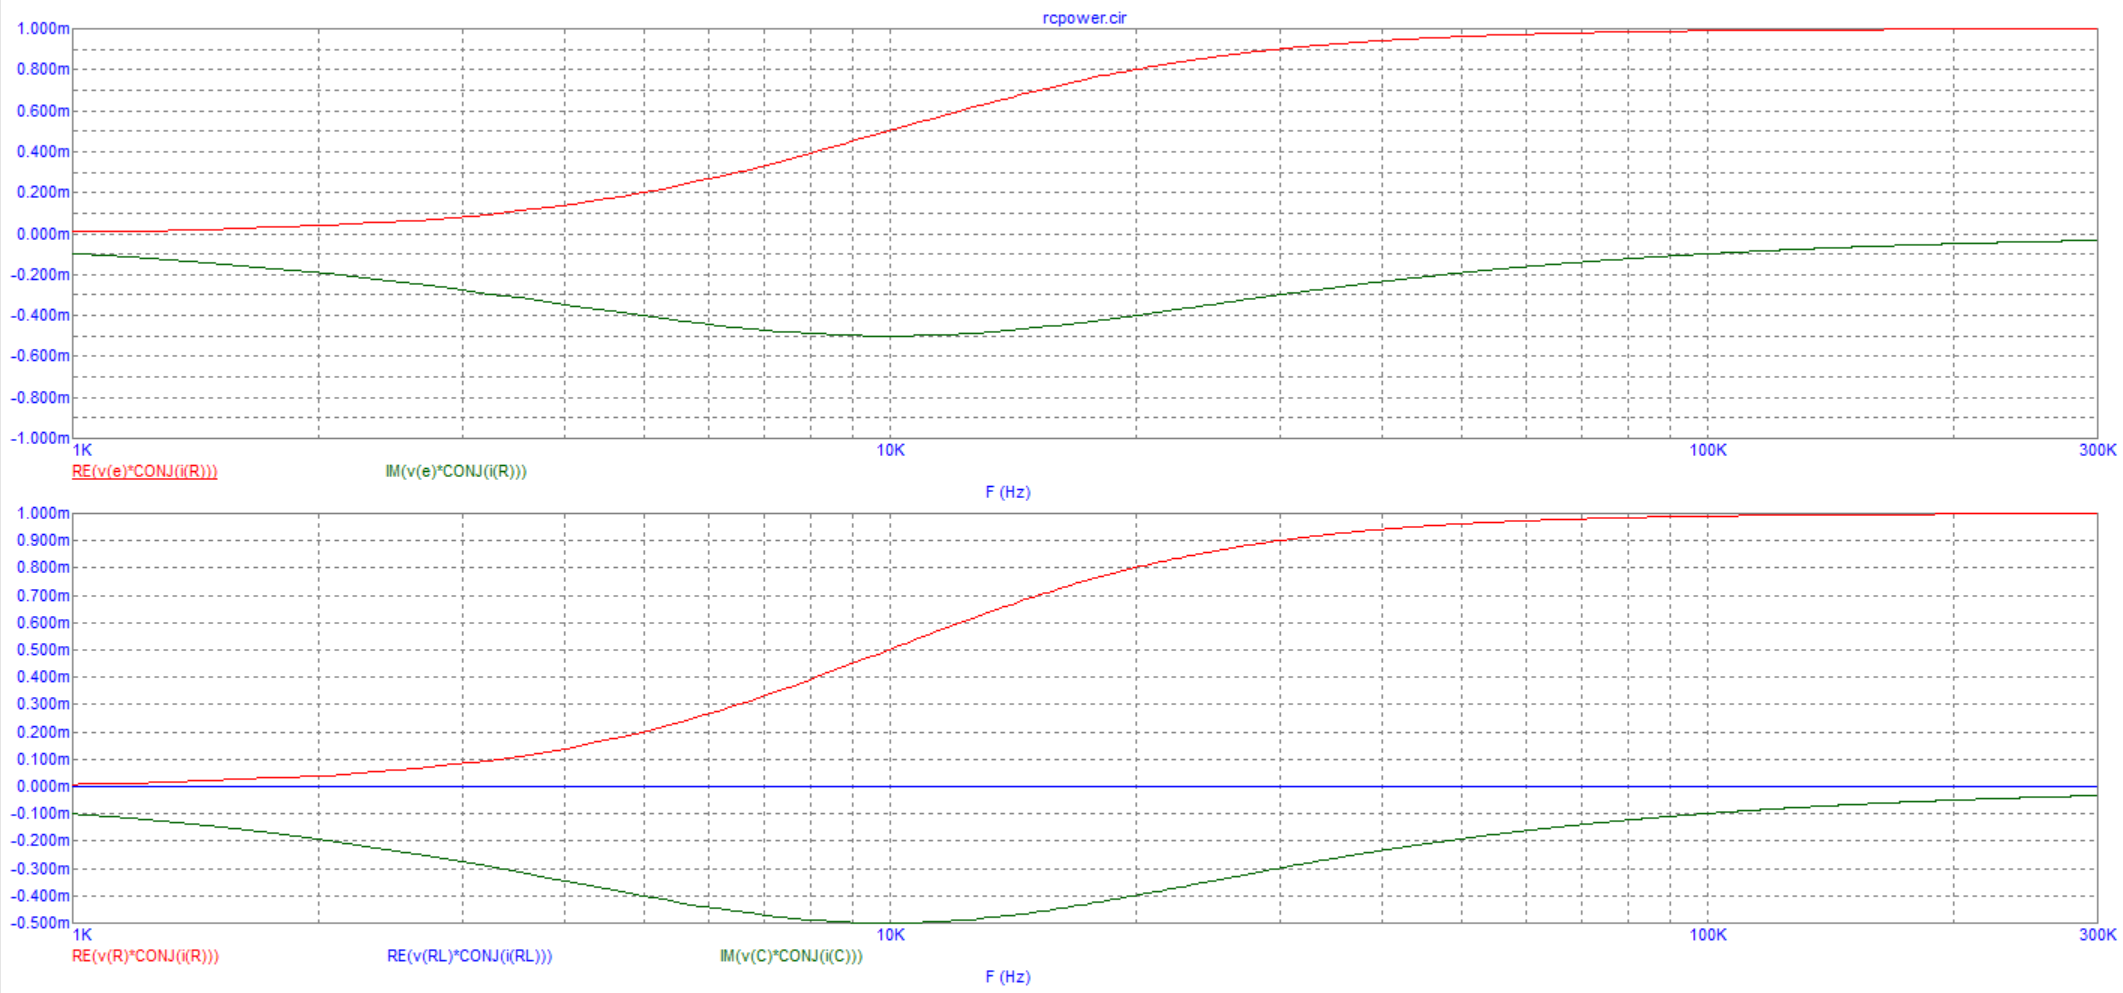
\includegraphics[scale=0.4]{rcpower_AC1.png}
\label{fig:Image1}
\end{figure}

Видно, что у реактивной компоненты потребление становится максимальным при частоте $f_0 = 10 \: kHz$, и стремится к нулю при частоте $f = 0$ и $f = \infty$. При $f = f_0$ выполняется закон сложения мощностей.

Подключая и отключая резитор $R_L$ варьированием $[1k, 1Meg \vert 1Meg] (1Meg = \infty)$, изучим его влияние на распределение мощностей в схеме при $f = f_0$.

\begin{figure}[H]
\centering
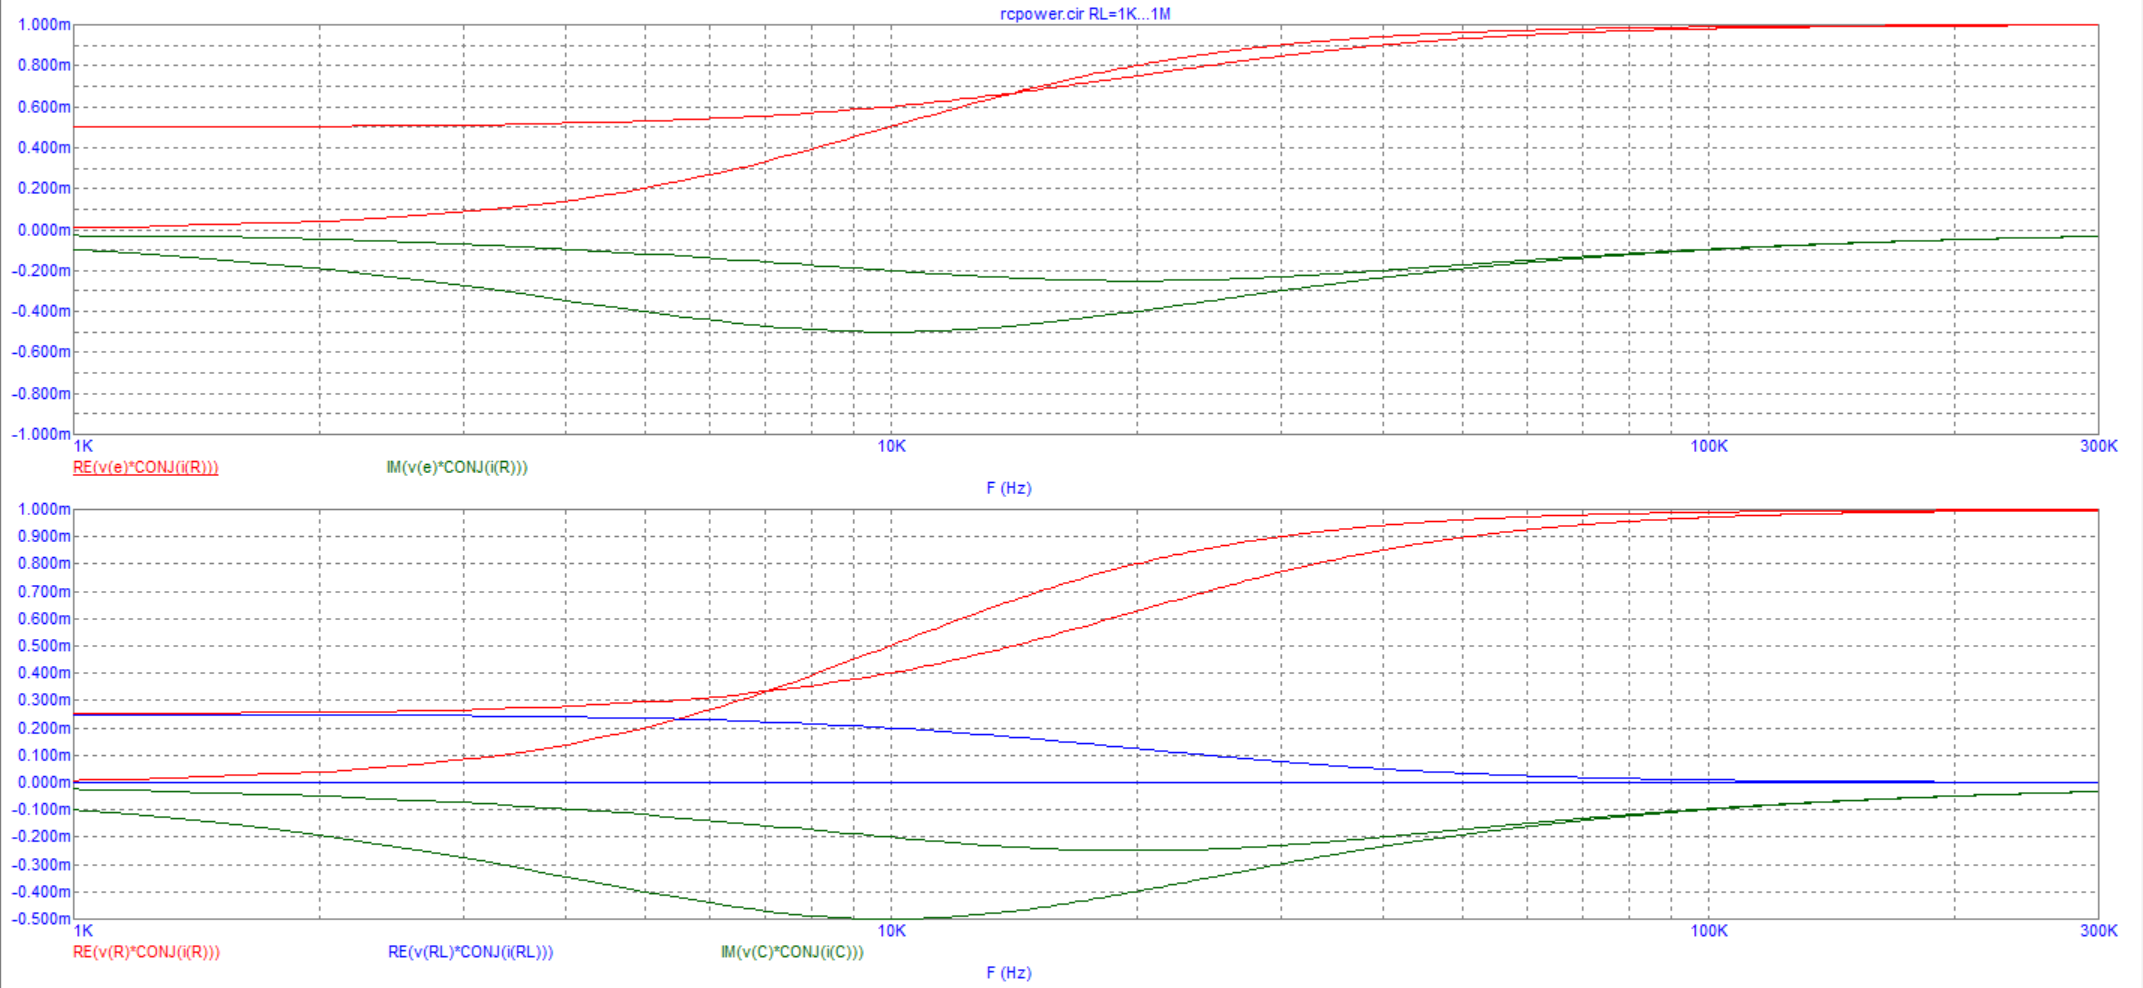
\includegraphics[scale=0.4]{rcpower_AC2.png}
\label{fig:Image1}
\end{figure}

При уменьшении значения сопротивления резистора $R_L$, его мощность возрастает до 0,2 mW, мощность на резисторе $R$ падает до 0,4 mW, а реактивная мощность конденсатора . Скорость увеличения мощности на резисторе $R_L$ становится равной -0,2 mW.

\section{Задание 2}
Откроем модель \textbf{rc2pole.cir}. 
\subsection{}

\begin{figure}[H]
\centering
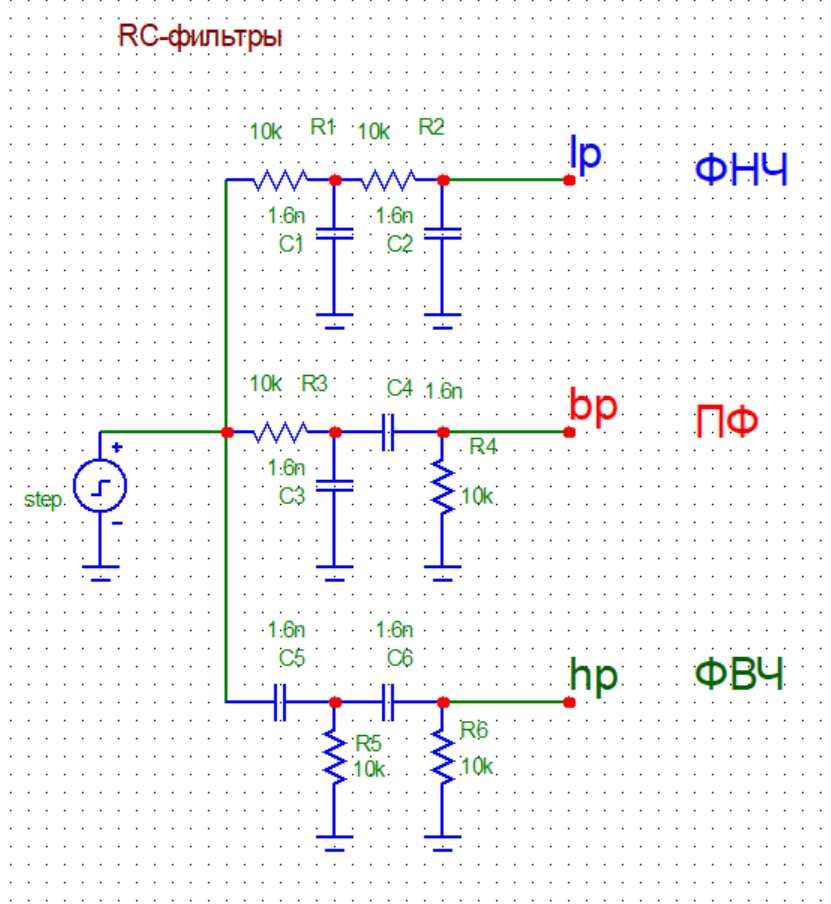
\includegraphics[scale=0.4]{rc2pole_img.png}
\label{fig:Image1}
\end{figure}

\begin{figure}[H]
\centering
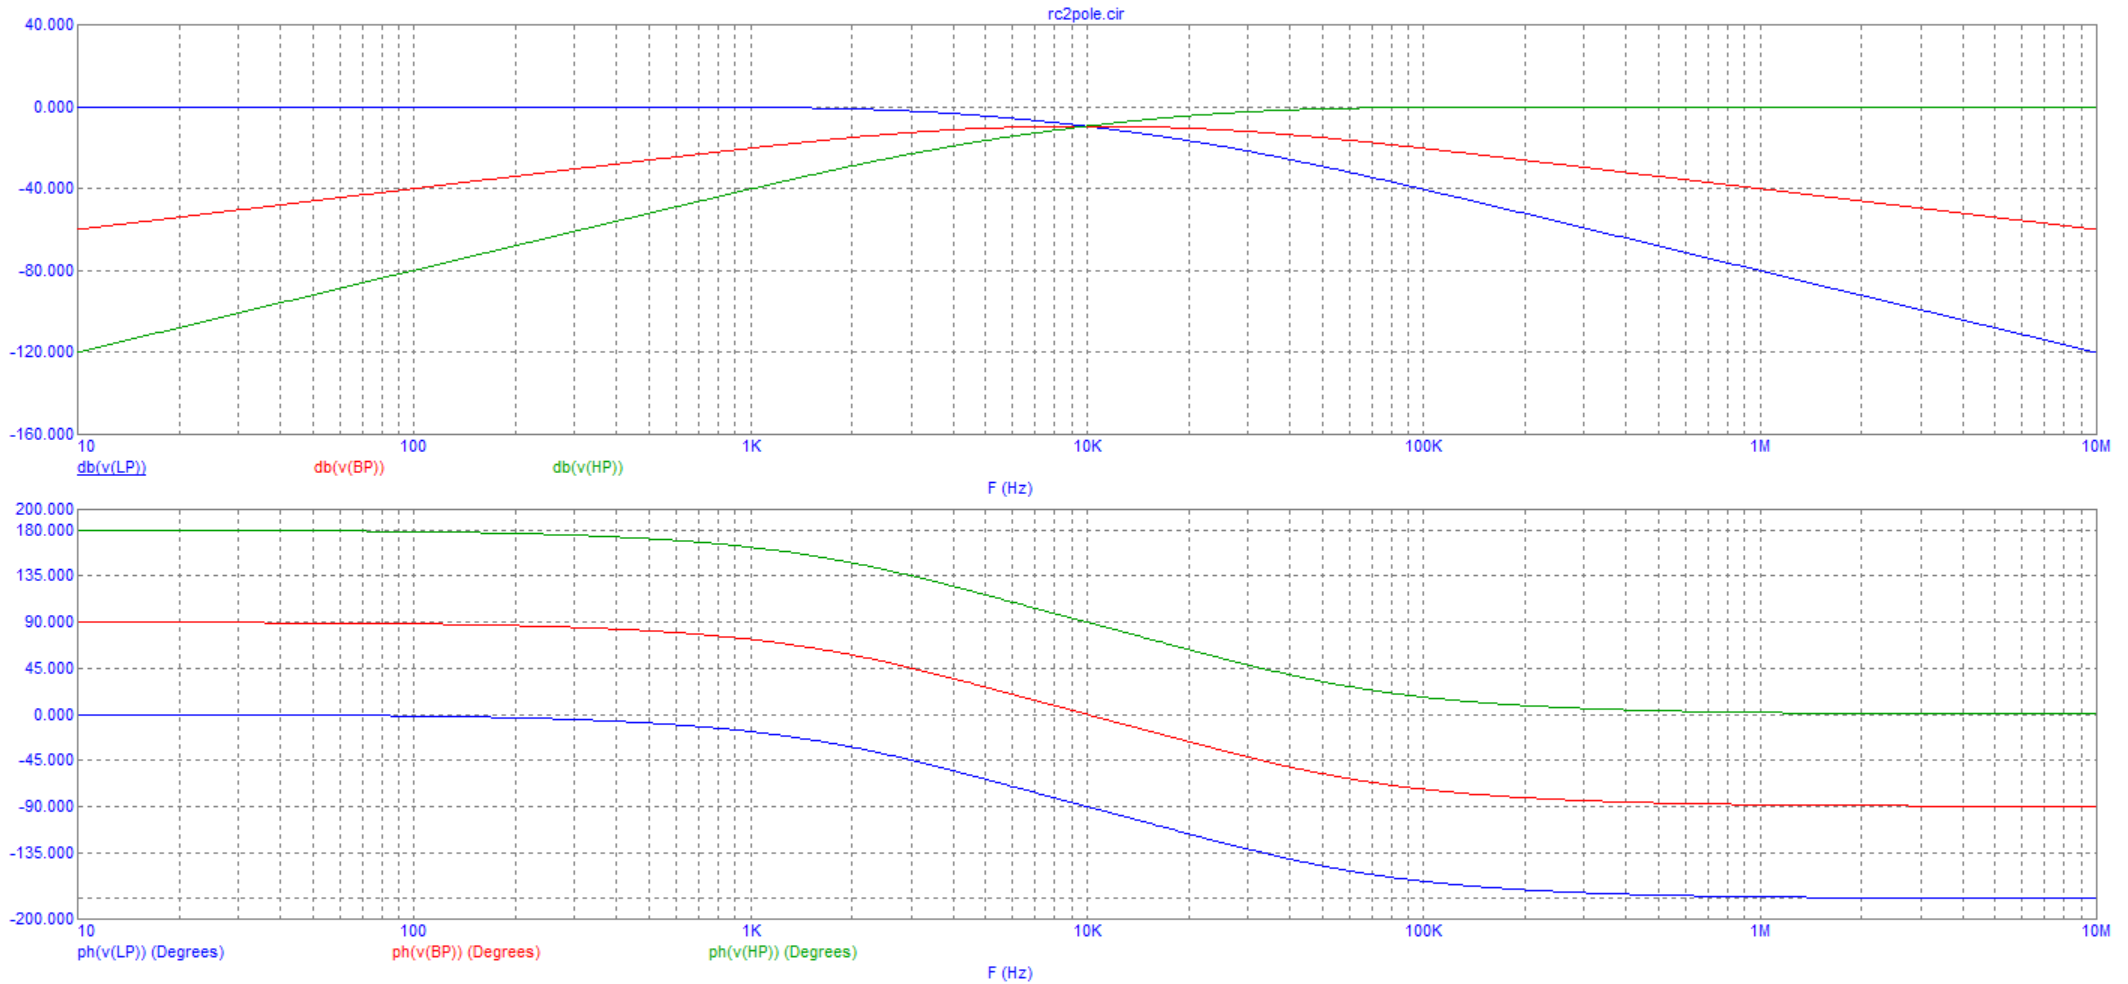
\includegraphics[scale=0.4]{rc2pole_AC.png}
\label{fig:Image1}
\end{figure}

По графикам определим затухание на частоте $f_0 \simeq 10 \: kHz$, оно равно -9,6 dB и скорость его нарастания в полосах задержания -40,4 + 9,6 = -30,8 dB/decade. По графикам  ФЧХ измерим значения фазовых сдвигов  ФВЧ, ПФ и ФНЧ на частотах 0, $f_0$, $\infty$.

\begin{center}
\begin{tabular}{|c|c|c|c|}
\hline 
 & ФВЧ & ПФ & ФНЧ \\ 
\hline 
0 & 180 & 90 & 0 \\ 
\hline 
$f_0$ & 90 & 0 & -90 \\ 
\hline 
$\infty$ & 0 & -90 & -180 \\ 
\hline 
\end{tabular} 
\end{center}

Двухсторонняя полоса $\triangle f$ пропускания ПФ $\approx$ 30 kHz, что в три раза больше $f_0$. Это сходится с теорией.

\subsection{}
Откроем графики преходных характеристик.

Оценим время спада $\tau_-$ первого выброса переходной характеристик ФВЧ до уровня $1/e \simeq 0,37$:

\[\tau_-= 5 \: \mu s\]

Оценим время нарастания $t_+$ фронта переходной характеристики ФНЧ до уровня $1 - 1/e \simeq 0,63$:

\[\tau_+ = 61 \: \mu s\]

Найдем их отношение:

\[\frac{\tau_+}{\tau_-} = 12,2\]

\section {Задание 3}
\subsection{}
Откроем модель \textbf{phshift.cir}.

\begin{figure}[H]
\centering
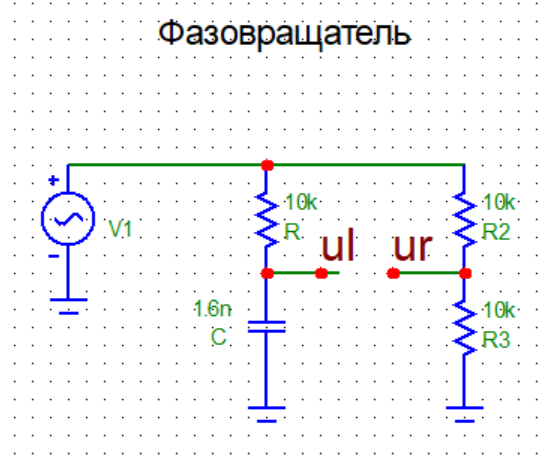
\includegraphics[scale=0.4]{phshift_omg.png}
\label{fig:Image1}
\end{figure} 

\begin{figure}[H]
\centering
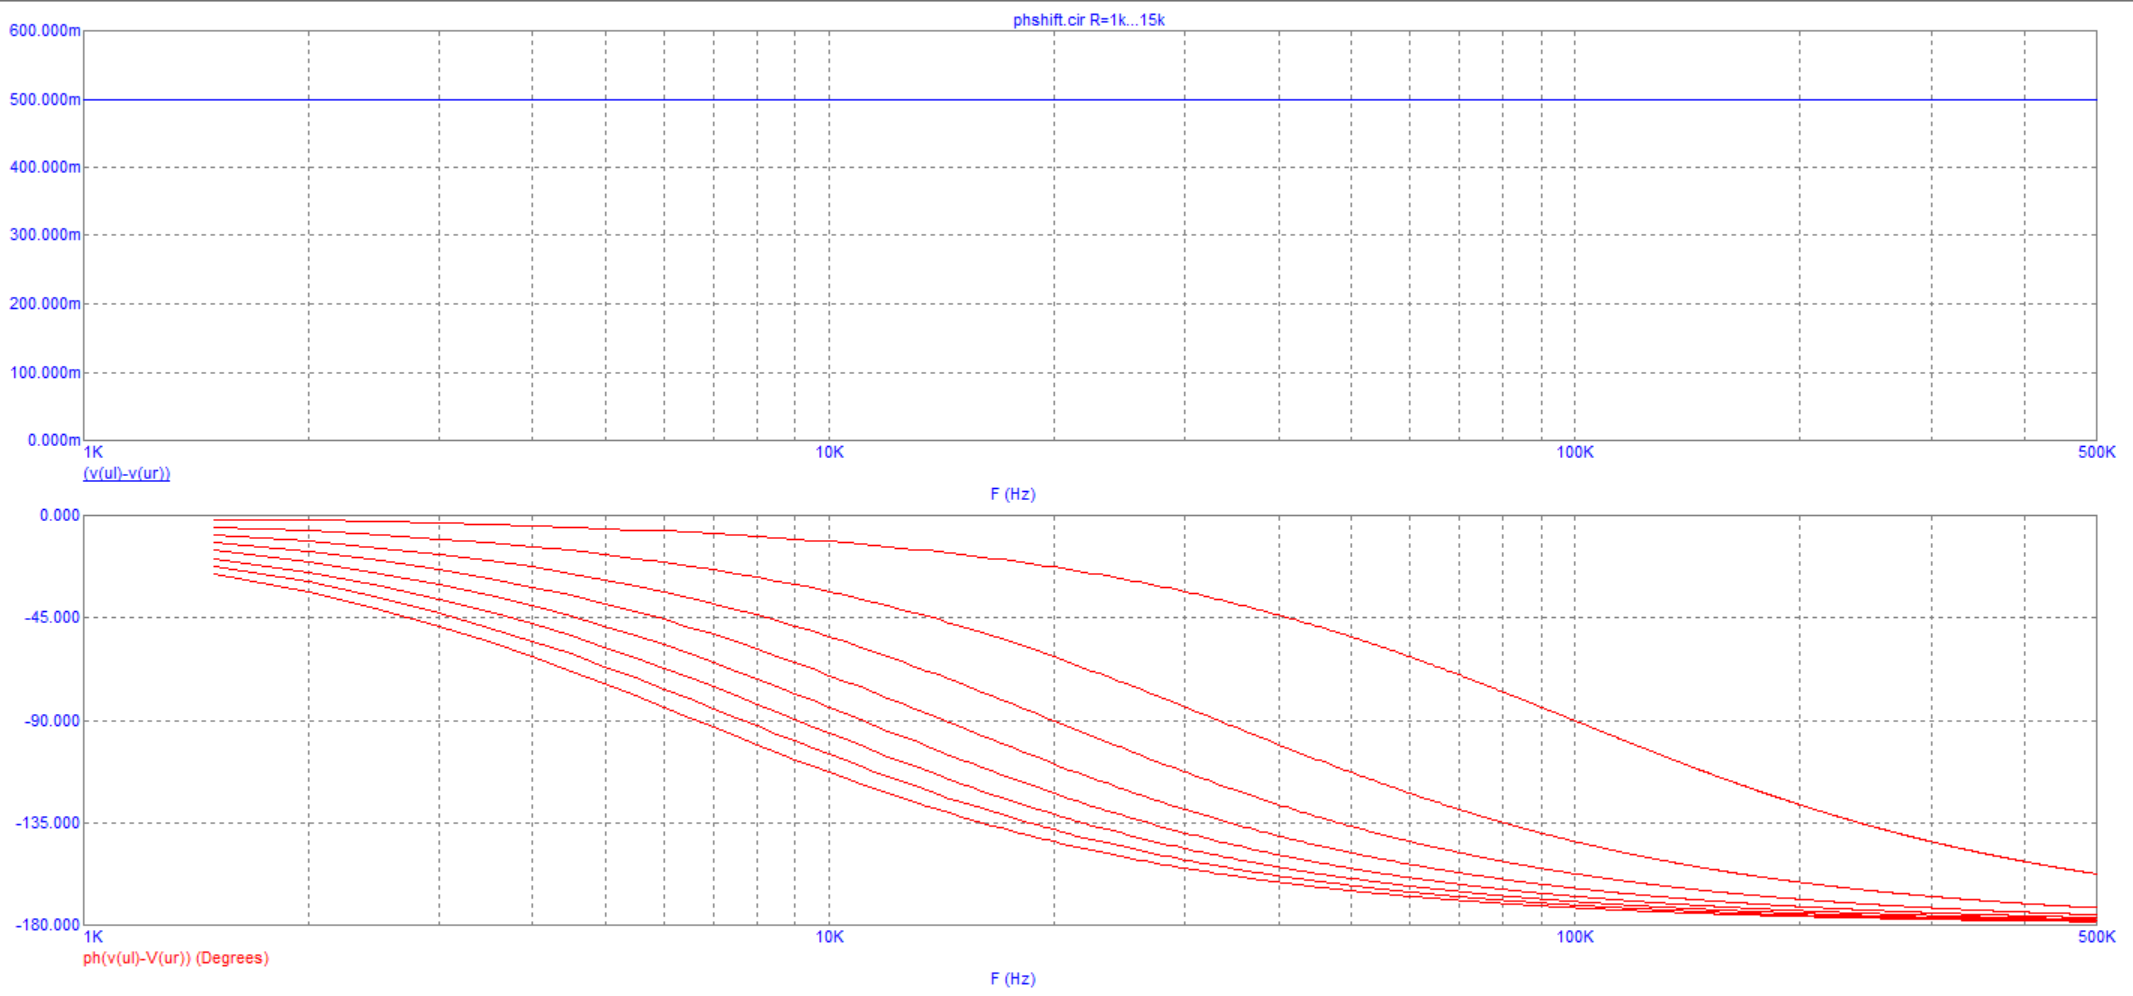
\includegraphics[scale=0.4]{phshift.png}
\label{fig:Image1}
\end{figure}

Наибольший диапазон перестройки реализуется на частоте $f = 20  \: kHz$. Границы этого диапазона $[-143,4; -22,7]$.

\subsection{}
Откроем модель двойного T-моста \textbf{2tbridge.cir}.

\begin{figure}[H]
\centering
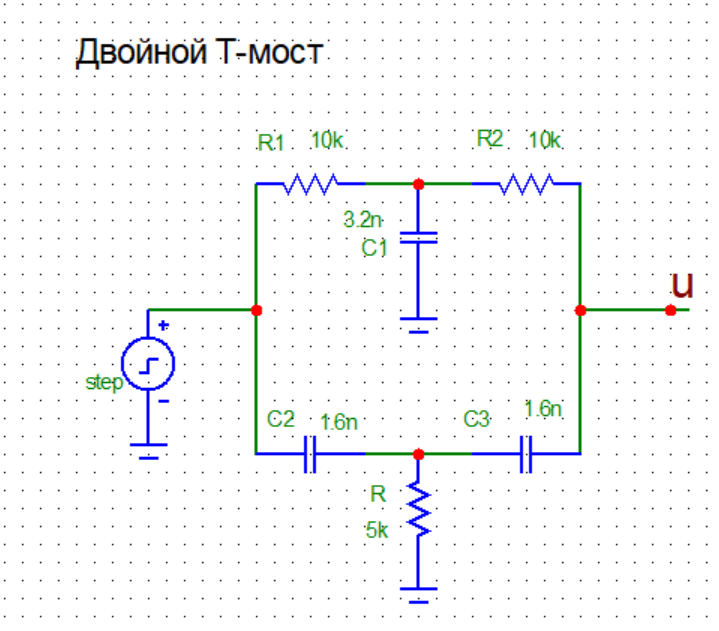
\includegraphics[scale=0.4]{2tbridge_img.png}
\label{fig:Image1}
\end{figure}

\begin{figure}[H]
\centering
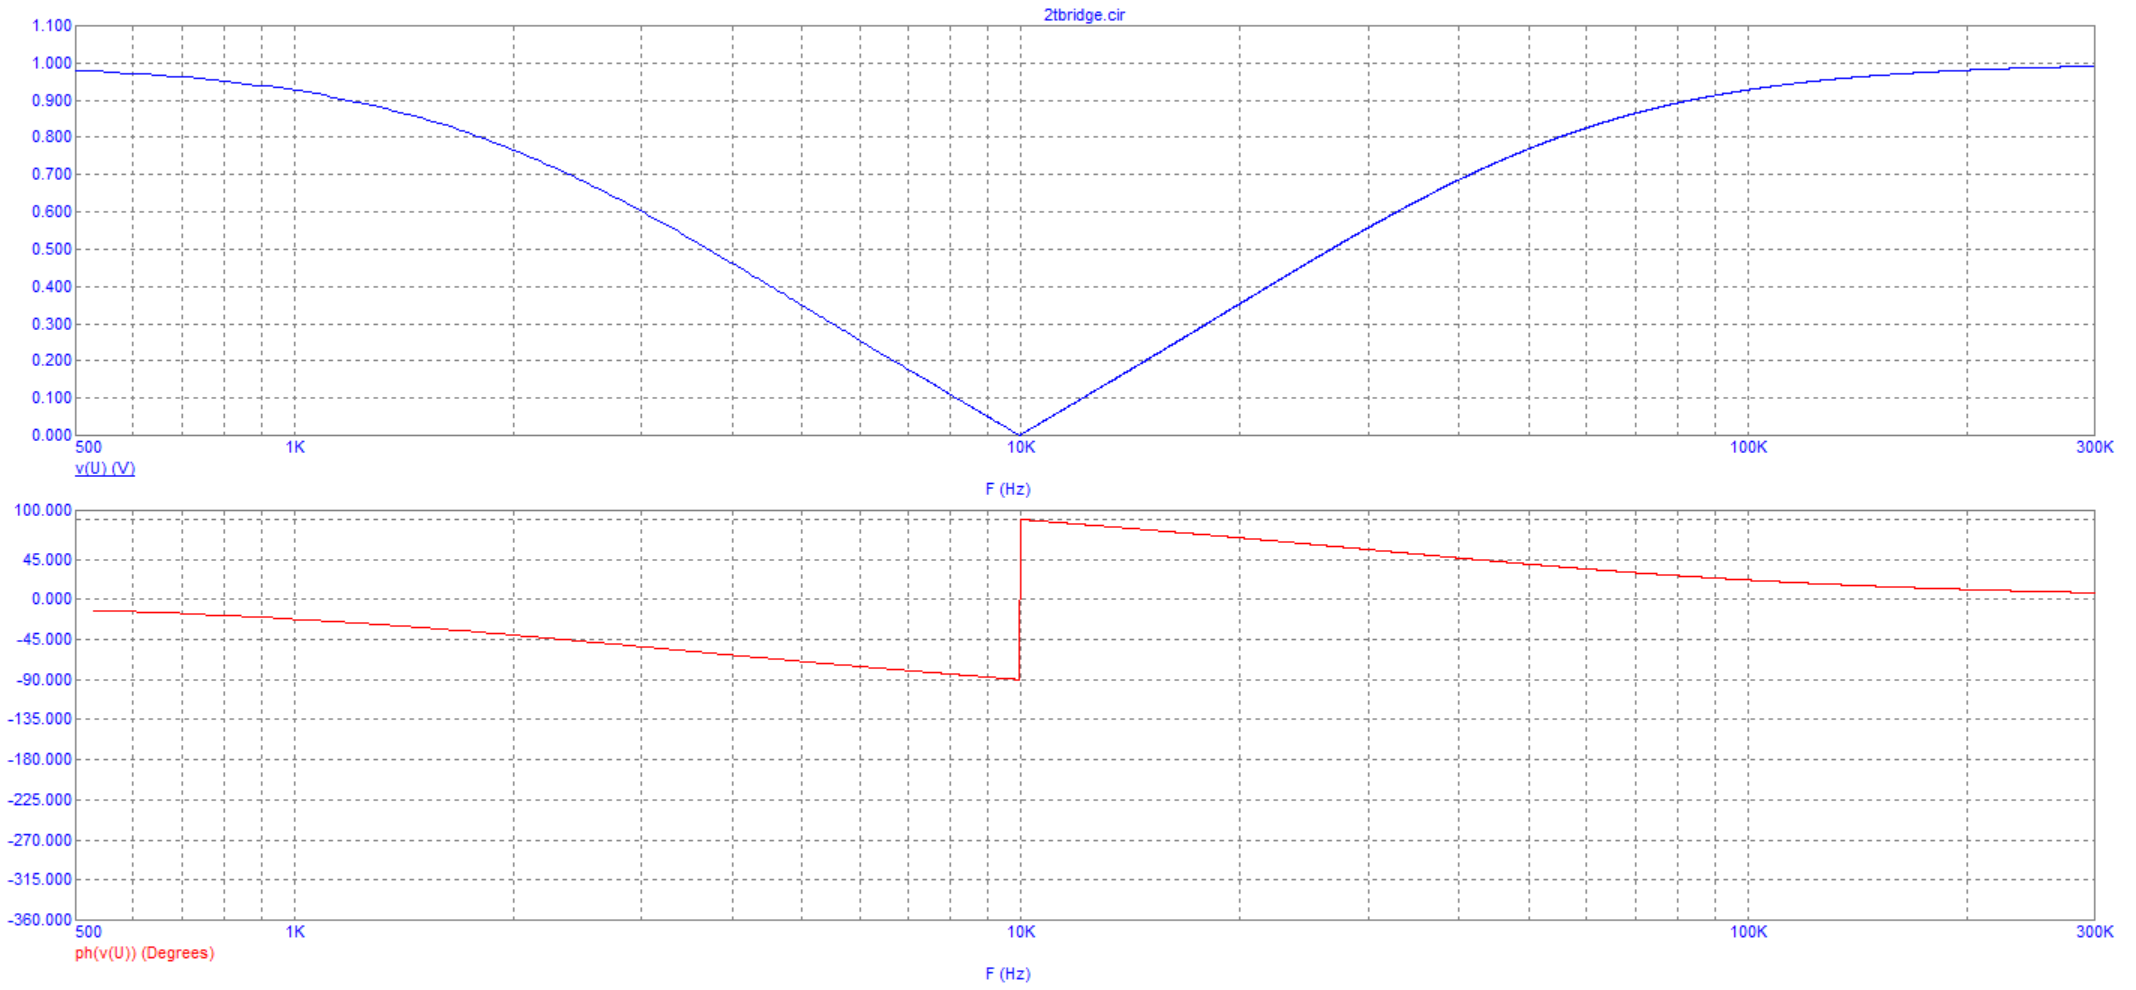
\includegraphics[scale=0.4]{2tbridge.png}
\label{fig:Image1}
\end{figure}

Измерим полосу режекции $\triangle f = 39 \: kHz$. $f_0 = 10 \: kHz$, следовательно выполняется $\triangle f = f_0$.

\begin{figure}[H]
\centering
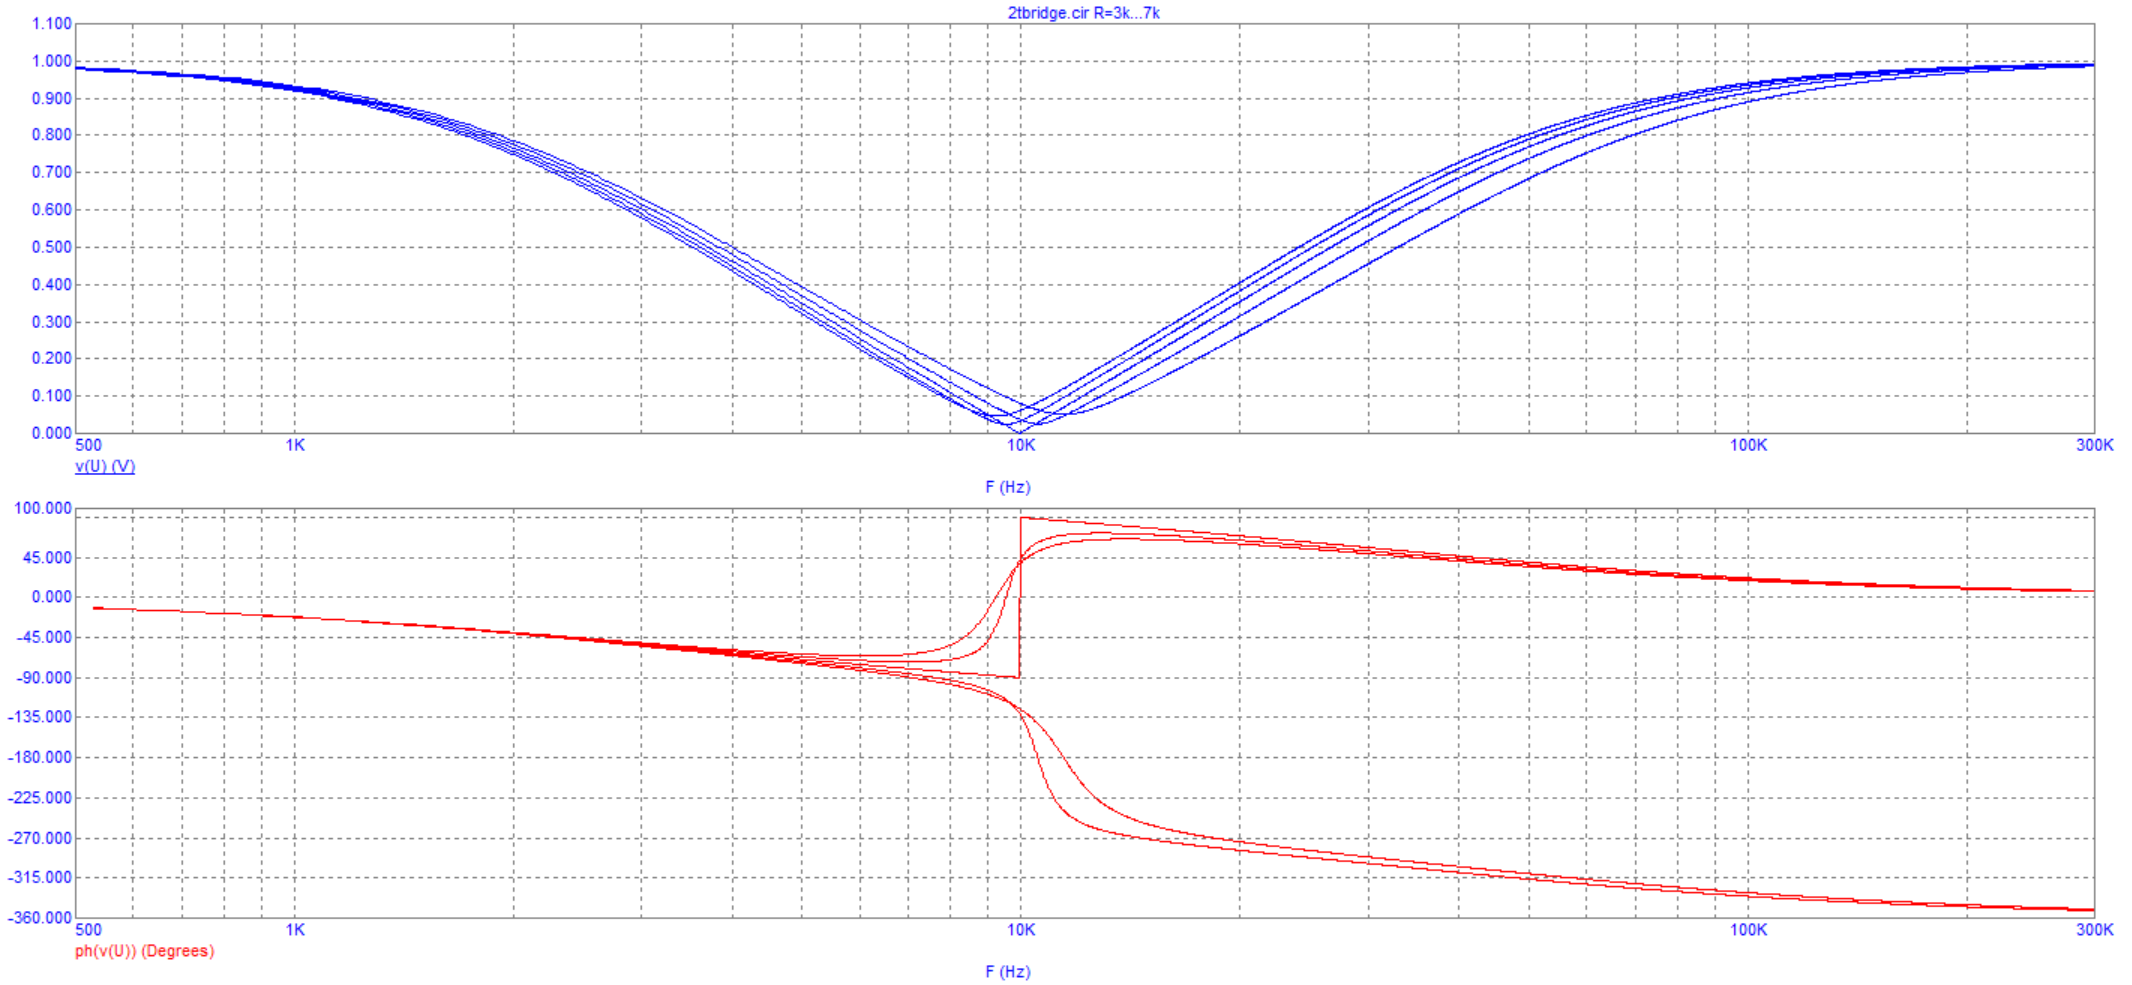
\includegraphics[scale=0.4]{2tbridge_AC2.png}
\label{fig:Image1}
\end{figure}

\begin{figure}[H]
\centering
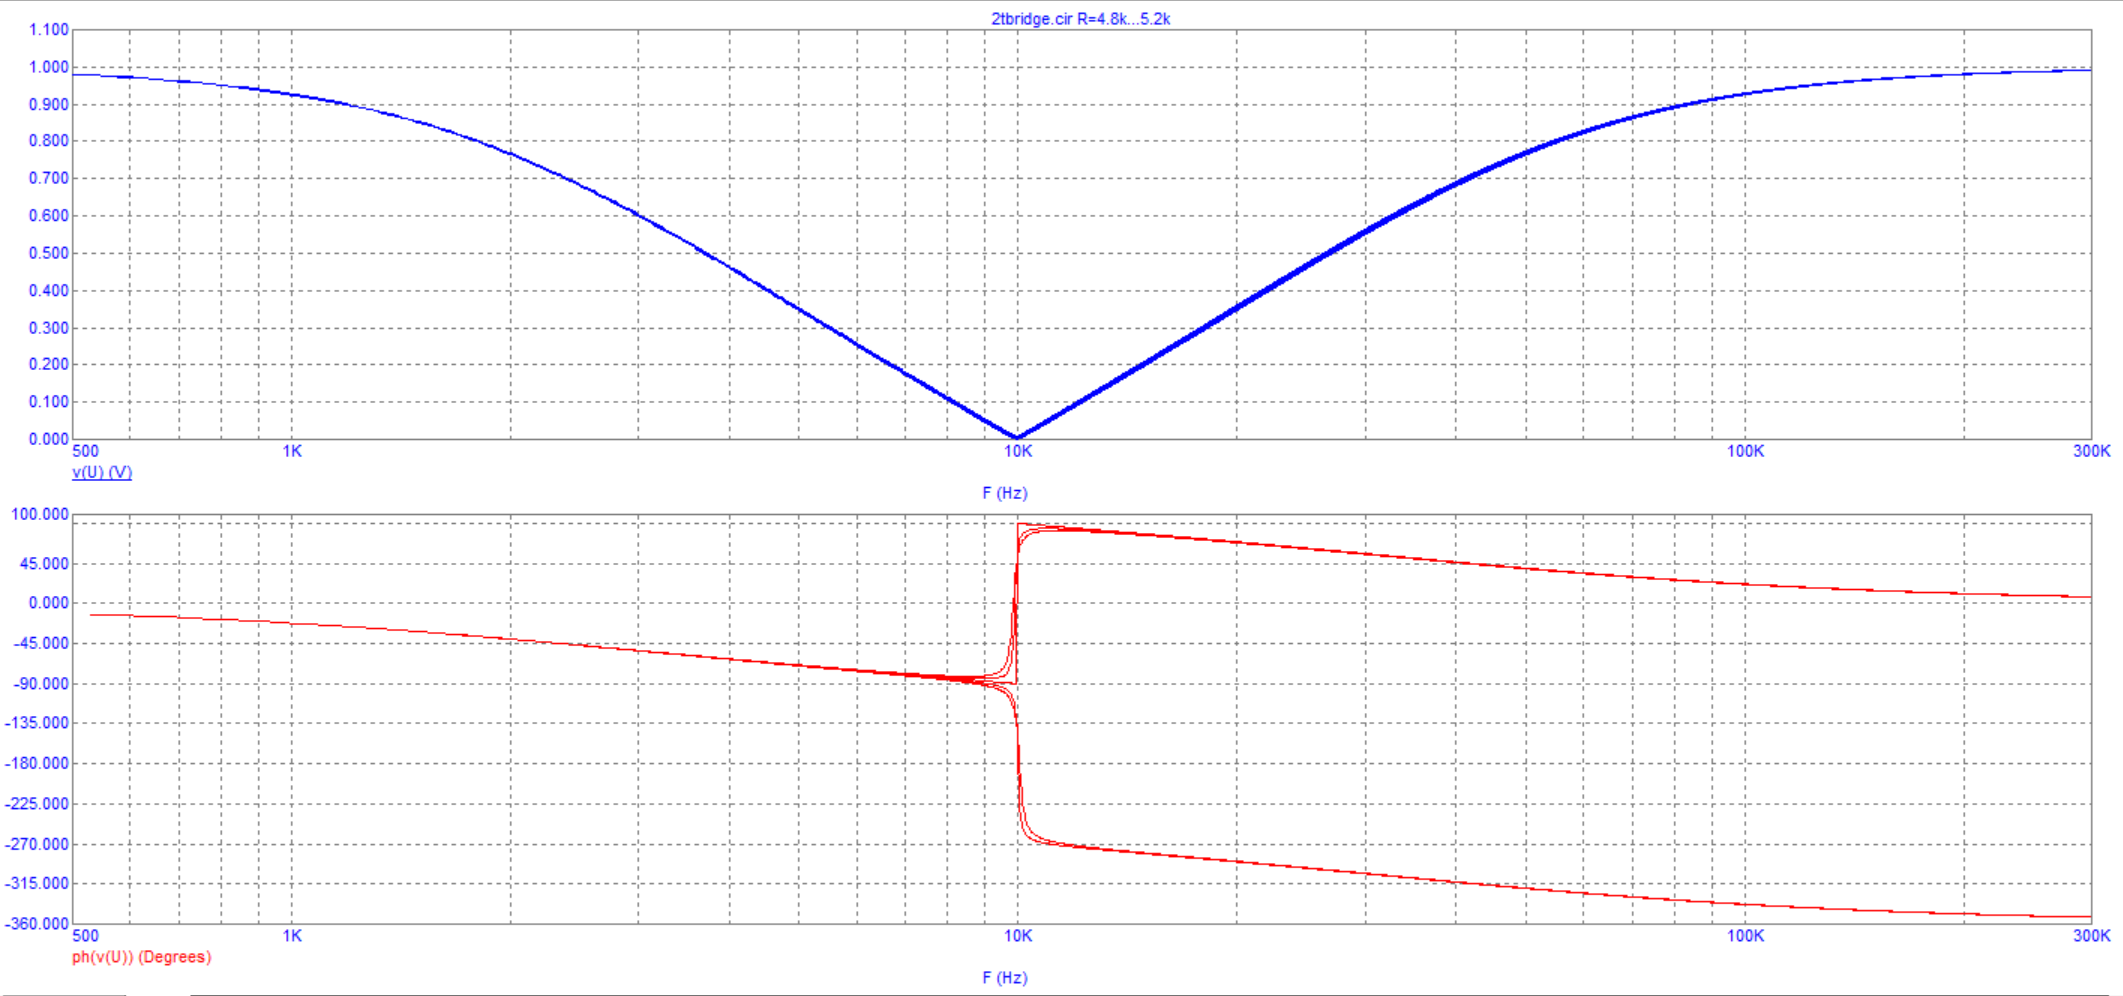
\includegraphics[scale=0.4]{2tbridge_AC3.png}
\label{fig:Image1}
\end{figure}

При росте $R$, $f_0$ падает. При $R = 5 \: k\Omega$ наблюдается скачок на ФЧХ.

\subsection{}
Подключив ко входу источник прямоугольного импульса, проанализиурем переходную характеристику. $\tau_+ = 4 \: \mu s$, $\tau_- = 58 \: \mu s$. Это сходится с теоретическими значениями.

\begin{figure}[H]
\centering
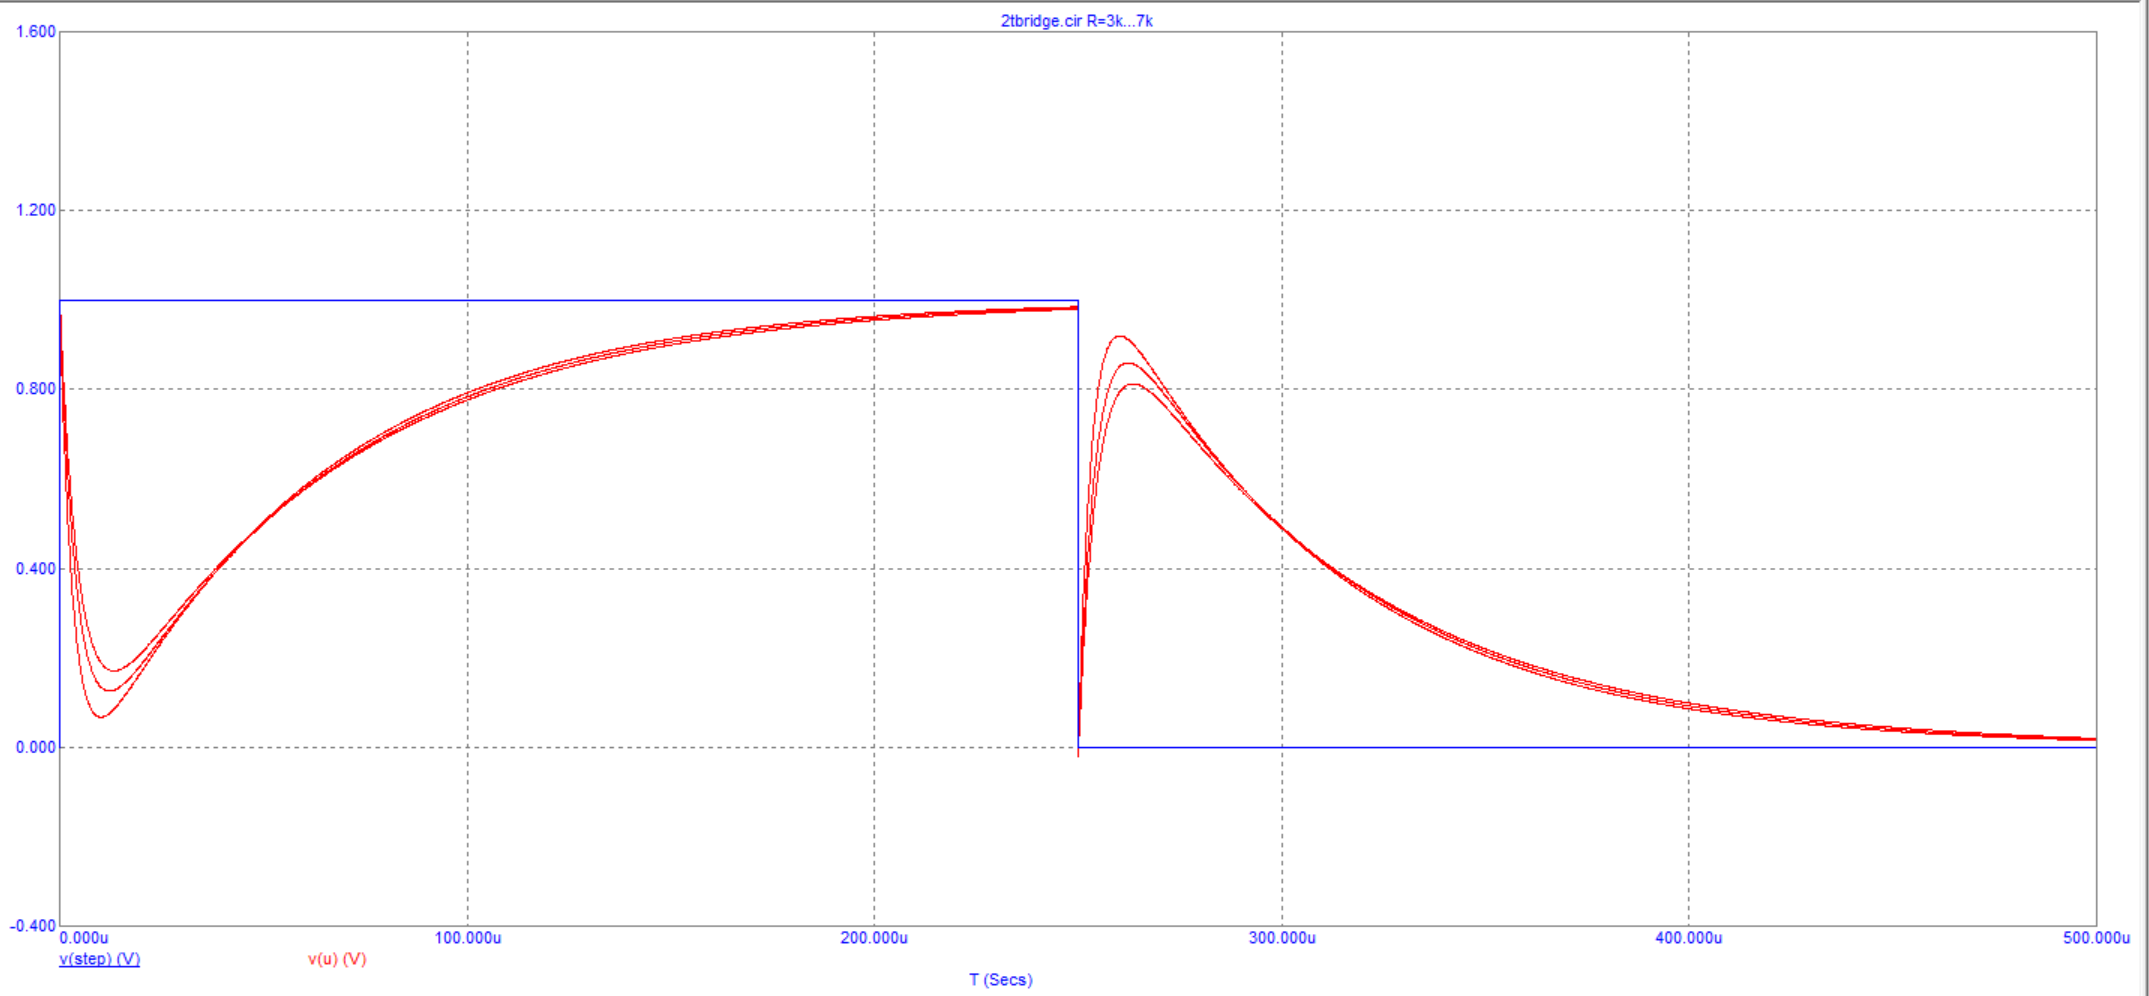
\includegraphics[scale=0.4]{2tbridge_AC4.png}
\label{fig:Image1}
\end{figure}

Варьирование приводит к усреднению функции.

\subsection{}

Откроем модель \textbf{2tdelay.cir}. 

\begin{figure}[H]
\centering
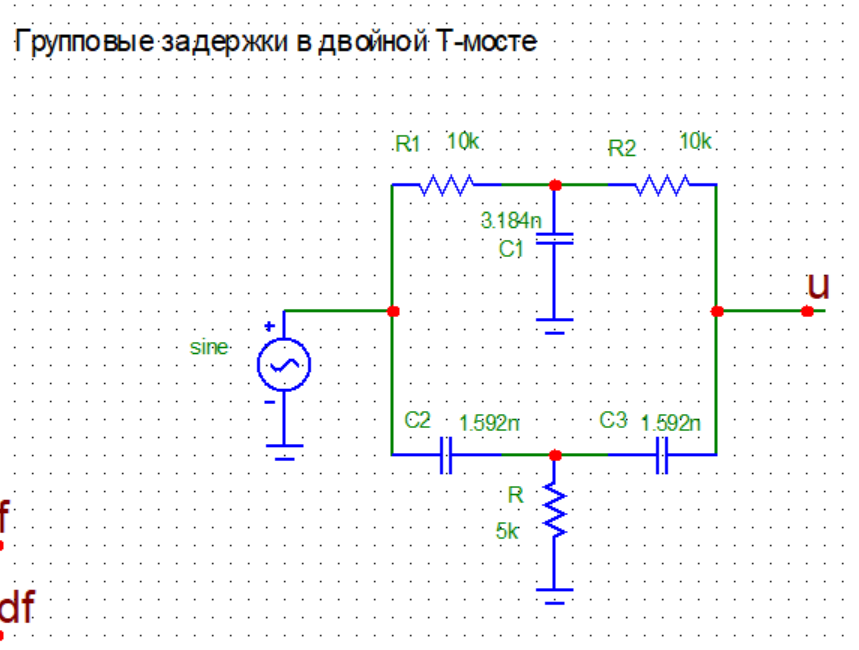
\includegraphics[scale=0.4]{2tdelay_img.png}
\label{fig:Image1}
\end{figure}

\begin{figure}[H]
\centering
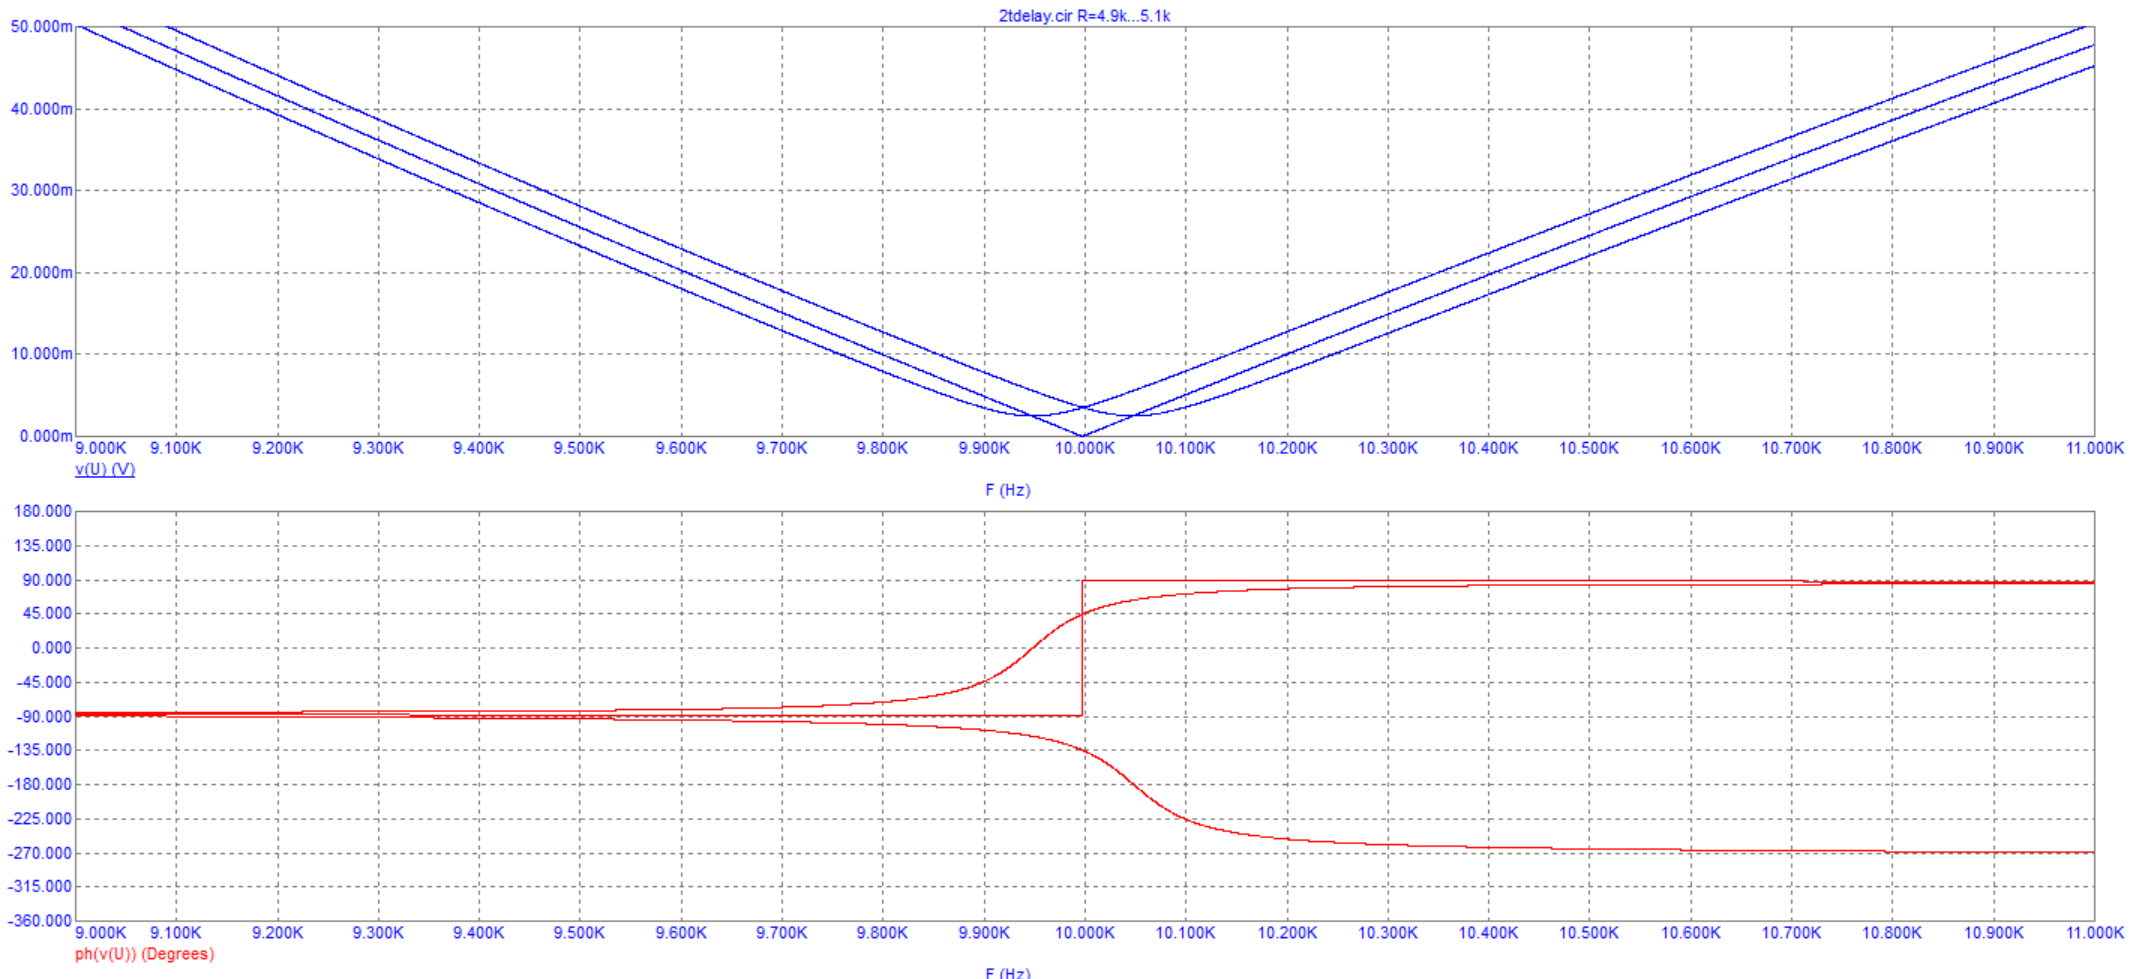
\includegraphics[scale=0.4]{2tdelay_AC1.png}
\label{fig:Image1}
\end{figure}

Оценим $Q = f_0/\triangle f$.

\begin{center}
\begin{tabular}{|c|c|c|c|}
\hline 
$R, \: k\Omega$ & 4,9 & 5 & 5,1 \\ 
\hline 
$f_0, \: kHz$ & 10,05 & 10 & 9,95 \\ 
\hline 
$\triangle f, \: kHz$ & 0,05 & $10^{-4}\cdot 2,5$ & 0,05 \\ 
\hline 
$Q$ & 100,5 & 40000 & 99,5 \\ 
\hline 
\end{tabular}
\end{center}

В режиме \textit{Transient} измерим групповые задержки $\tau_g$:

\[\tau_g = 3 \: ms,\]

значение для обоих случаев ($R = 4,9 \: k\Omega, f = 10,05 \: kHz$ и $R = 5,1 \: k\Omega, f = 9,95 \: k\Omega$).

\begin{figure}[H]
\centering
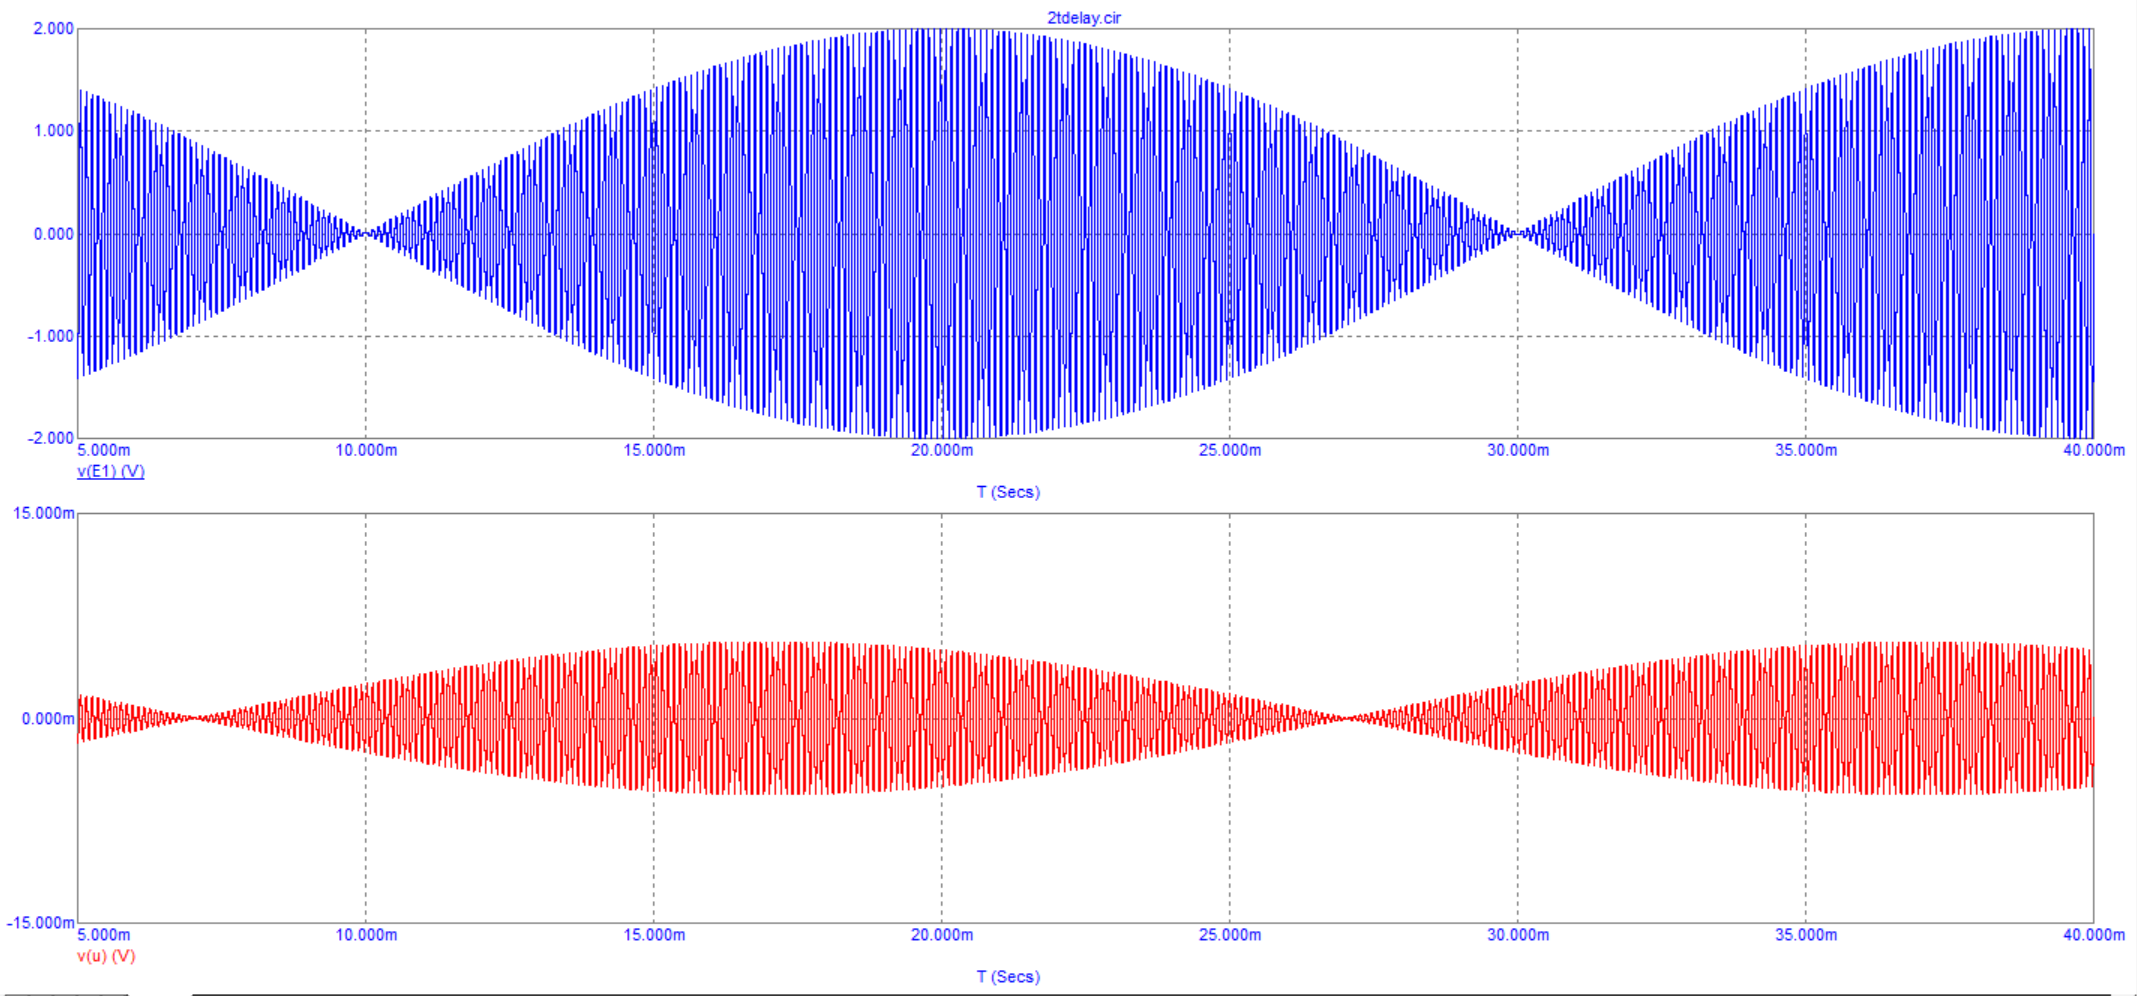
\includegraphics[scale=0.4]{2tdelay_AC2.png}
\label{fig:Image1}
\end{figure}

\section {Задание 4}


\subsection{}
На макетной плате соберем схему полосового фильтра (его схема, как и схема ФНЧ и ФВЧ представлены на рисунке).

\begin{figure}[H]
\centering
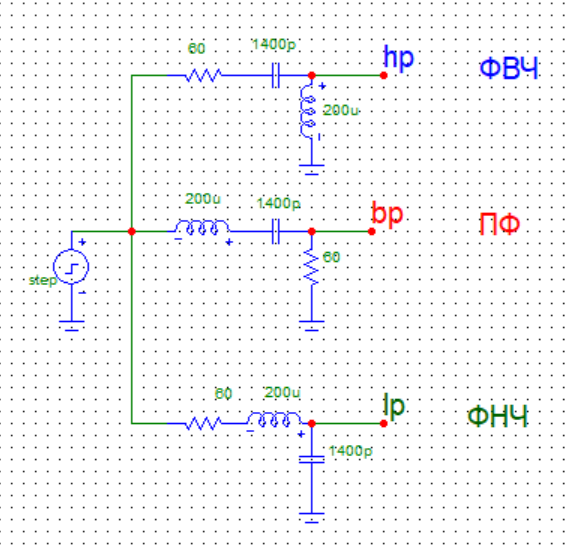
\includegraphics[scale=0.4]{rlc2pole_img.png}
\label{fig:Image1}
\end{figure}

\[L = 220 \: \mu H\]
\[C = 1 \: \mu F\]
\[r = 92 \: \Omega\]

Измерим резонансную частоту и коэффициент передачи:

\[f_0 = 366 \: kHz\]

\[\triangle f = 75 \: kHz\]

\[Q = \frac{f_0}{\triangle f} = 4,8\]

\subsection{}
Из тех же компонент соберем схемы ФВЧ и ФНЧ. Измерим для них резонансную частоту и отношения $K(f_0)/K(0)$ для ФНЧ и $K(f_0)/K(\infty)$ для ФВЧ.

\[Q = \frac{K(f_0)}{K(0)} = 5,18\]

\[Q = \frac{K(f_0)}{K(\infty)} = 4,1\]

\subsection{}
Подключим генератор прямоугольных импульсов. Изучим переходные характеристики ФВЧ, ФНЧ и ПФ. Прикинем по осцилограммам период колебаний и время их затухания до уровня $1/e = 0,37$ и дадим оценку резонансной частоты и добротности.

Для ФВЧ:

\[T = 2,8 \: \mu s\]

\[\tau = 0,45 \: \mu s\]

\[f_0 = 365 \: kHz\]

\[Q = 6,2\]

Для ФНЧ:

\[T = 2,83 \: \mu s\]

\[\tau = 0,49 \: \mu s\]

\[f_0 = 352 \: kHz\]

\[Q = 5,7\]

Для ФВЧ:

\[T = 2,84 \: \mu s\]

\[\tau = 0,51 \: \mu s\]

\[f_0 = 351 \: kHz\]

\[Q = 5,6\]

\subsection{}
Откроем в MicroCap модель \textbf{rlc2pole.cir}, изучим частотные фазовые и переходные характеристики фильтров.

\begin{figure}[H]
\centering
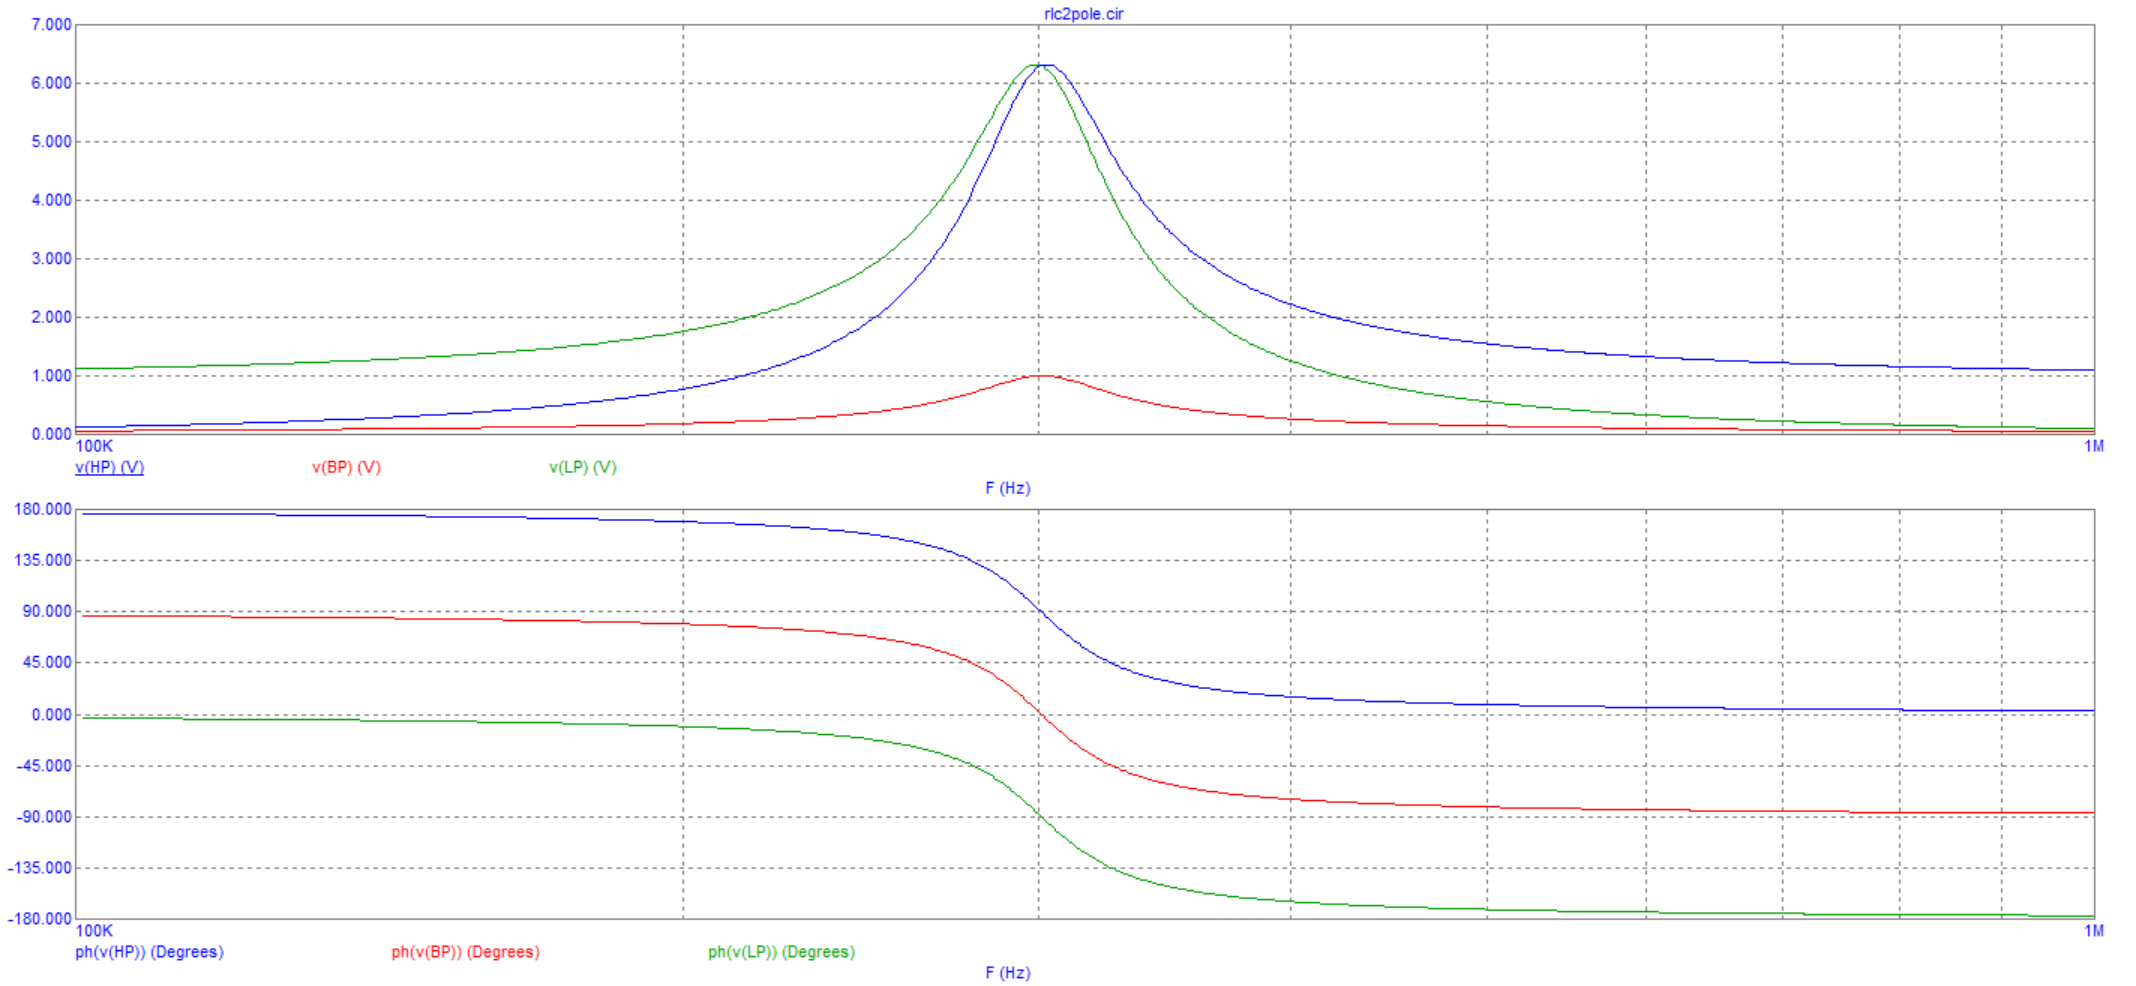
\includegraphics[scale=0.4]{rlc2pole_AC1.png}
\label{fig:Image1}
\caption{Частотные и фазовые характеристики}
\end{figure}

\begin{figure}[H]
\centering
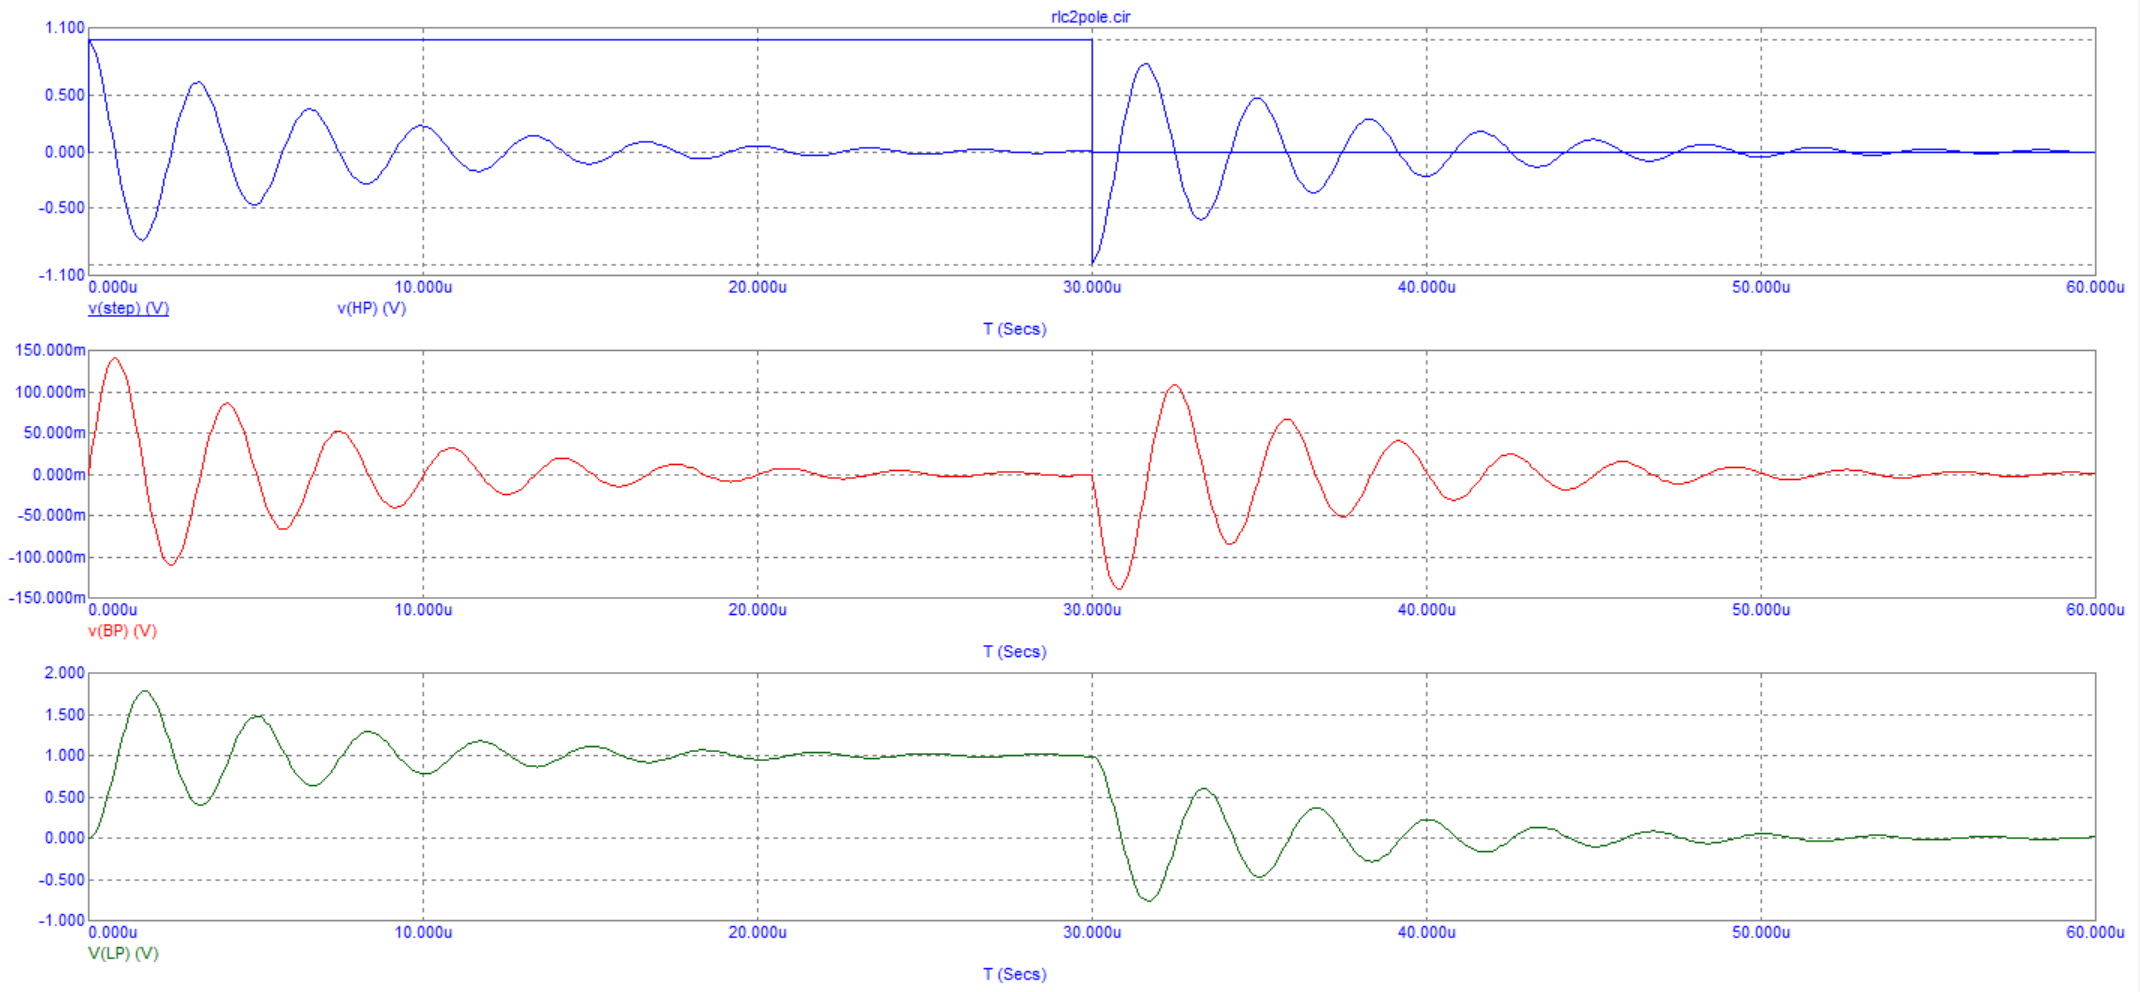
\includegraphics[scale=0.4]{rlc2pole_transient.png}
\label{fig:Image1}
\caption{Переходные характеристики}
\end{figure}

\subsection{}
Откроем модель \textbf{groupdel.cir} полосового фильтра. Наблюдая в режиме \textit{Transient} отклик на двухчастотный сигнал изучим зависимость групповой задержки $\tau_g$ от $R = 10, 20, 40, 100$.

\begin{center}
\begin{tabular}{|c|c|c|c|c|}
\hline 
$R, \: \Omega$ & 10 & 20 & 40 & 100 \\ 
\hline 
$\tau_g, \: ms$ & 0,5 & 0,29 & 0,152 & 0,064 \\ 
\hline 
$\tau_{\textit{th}}, \: ms$ & 0,62 & 0,31 & 0,155 & 0,06 \\ 
\hline 
Q & 195 & 98 & 49 & 19 \\ 
\hline 
\end{tabular}
\end{center}

\subsection{}
Откроем модель \textbf{lcpower.cir}.

\begin{figure}[H]
\centering
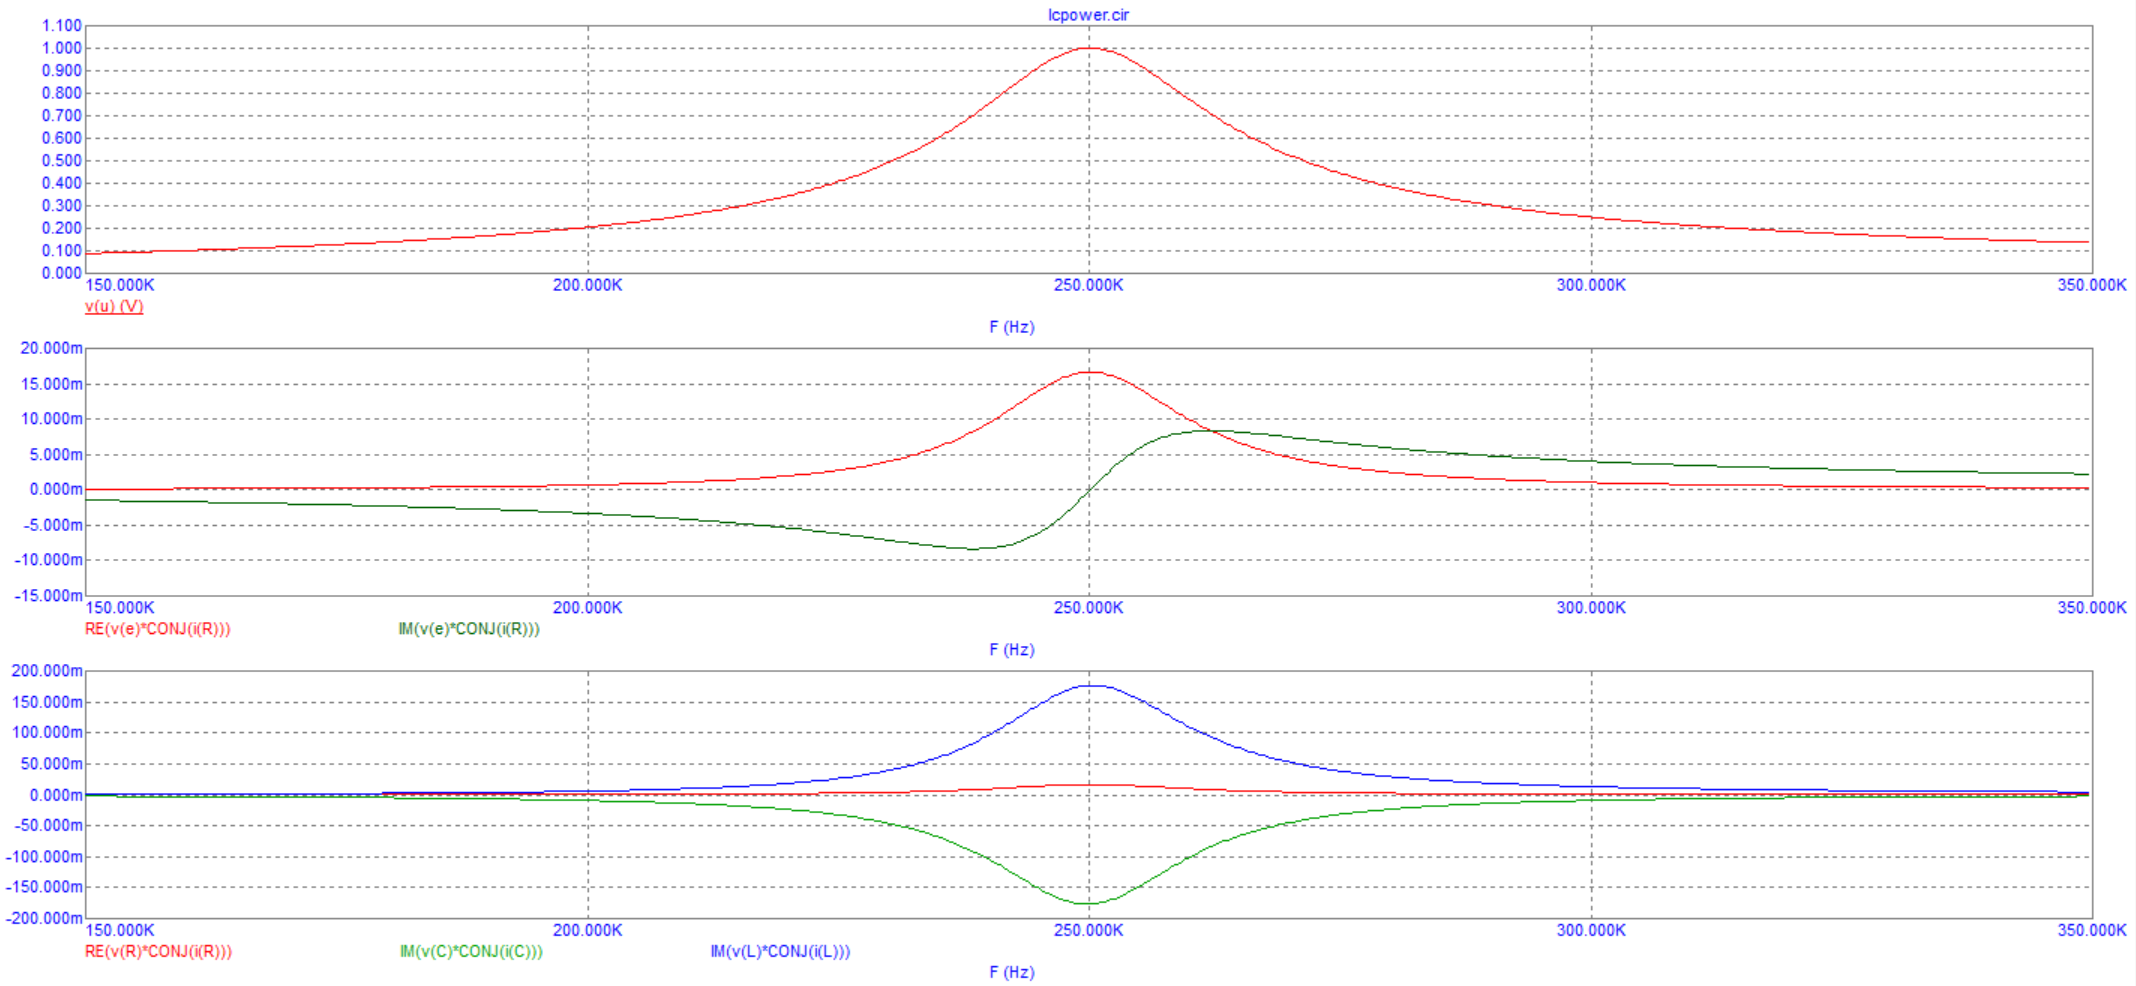
\includegraphics[scale=0.4]{lcpower.png}
\label{fig:Image1}
\end{figure} 

На частоте резонанса $f_0 = 250 \: kHz$.

\[P_L = 176,066 \: m \quad P_C = -177,477 \: m \quad P_R = 15,89 \: m \Rightarrow \sum P = 14,47\]

\[P_{\sum \textit{th}} = 16,18 \: m\]

На одной из границ полосы пропускания $f_1 = 238 \: kHz$:

\[P_L = 116,577 \: m \quad P_C = -122,51 \: m \quad P_R = 11,14 \: m \Rightarrow \sum P = 5,147\]

\[P_{\sum \textit{th}} = 11,367 \: m\]

Закон суммирования выполняется.

\section{Задание 5}

\subsection{}

Откроем в MicroCap модель \textbf{parallel.cir} параллельного контура с $f_0 = 100 \: kHz$, $\varrho = 570$. По схеме оценим параметры:

\[\alpha = \frac{\rho}{R_0}\]

\[\beta = \frac{R}{\rho}\]

\[Q = \frac{1}{\alpha + \beta}\]

\begin{figure}[H]
\centering
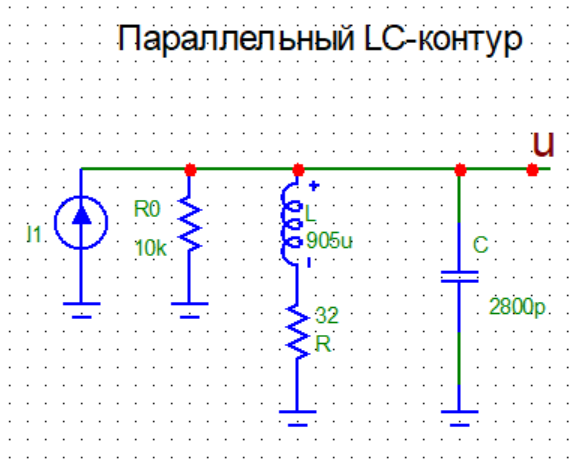
\includegraphics[scale=0.4]{parallel_img.png}
\label{fig:Image1}
\end{figure} 

\[\rho = \sqrt{\frac{L}{C}} = 568\]

\[\alpha = 0,0568 \quad \beta = 0,0563\]

\[Q = 8,84\]

\subsection{}
Найдем резонансную частоту $f_0 = 100 \: kHz$, полосу пропускания $\Delta f = 11,6 \: kHz$. Измерим сопротивление контура $R_0 = 5 \: k\Omega$. Оценим добротность как:

\[Q = \frac{R_0}{\rho} = 8,8\]

\[Q = \frac{f_0}{\triangle f} = 8,6\]

\subsection{}
Изучим влияние на добротность последовательных потерь $R$, установив варьирование $R = [0, 32 \Vert 32]$. 

\begin{figure}[H]
\centering
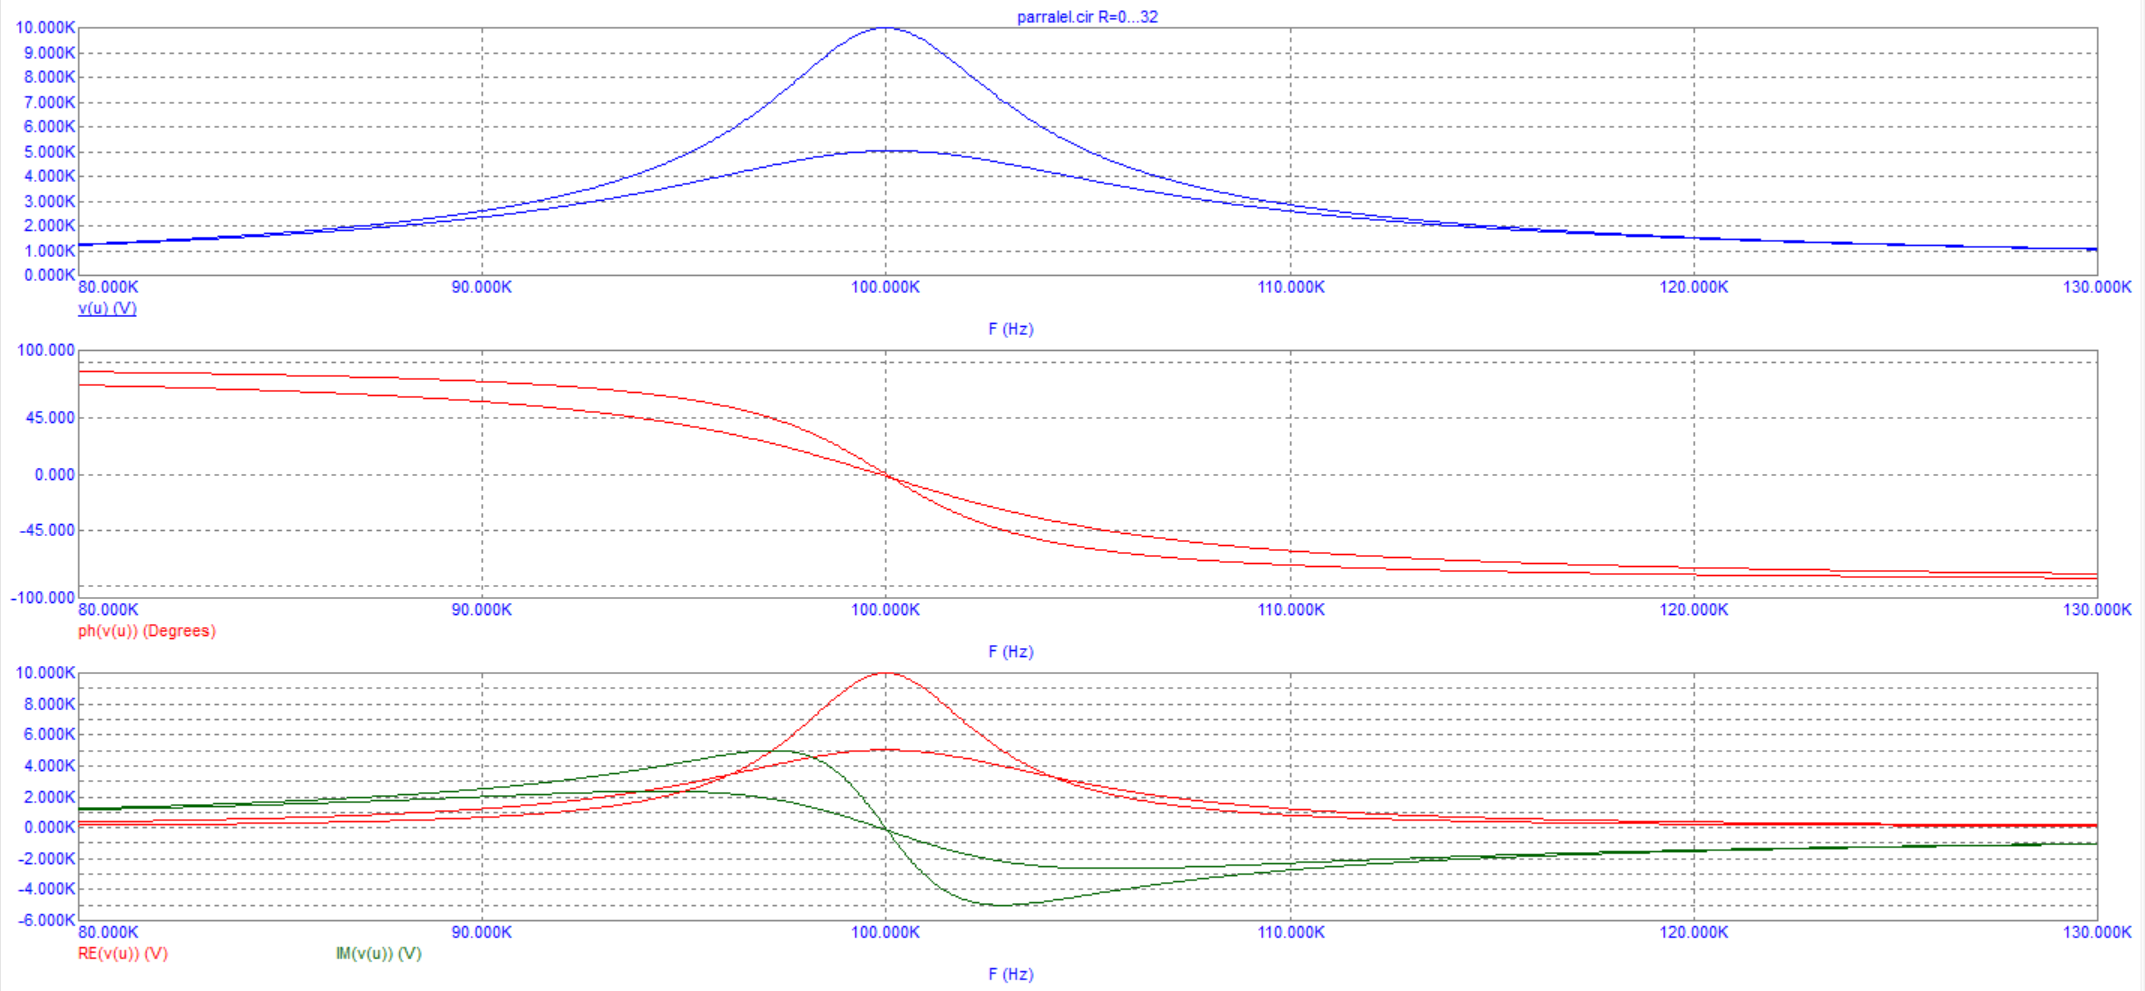
\includegraphics[scale=0.4]{parallel_AC1.png}
\label{fig:Image1}
\end{figure} 

Добротность при $R = 0$:

\[Q = \frac{f_0}{\triangle f} = 17,3\]

Изучим влияние параллельных потерь $R_0$, установив варьирование $R_0 = [10k, 1000k \Vert 1000k]$. Измерим добротность при $R_0 = 1000 \: k\Omega$:

\[Q = \frac{f_0}{\triangle f} = 17,2\]

При увеличении $R$ от 0 \Omega до 32 \Omega $1/Q$ меняется от 0,058 до 0,116. При увеличении $R_0$ от 10 \Omega до 1000 \Omega $1/Q$ меняется от 0,116 до 0,058.

\subsection{}
Изучим зависимость частоты параллельного резонанса от $R = [0, 150 \Vert 50]$.

\begin{figure}[H]
\centering
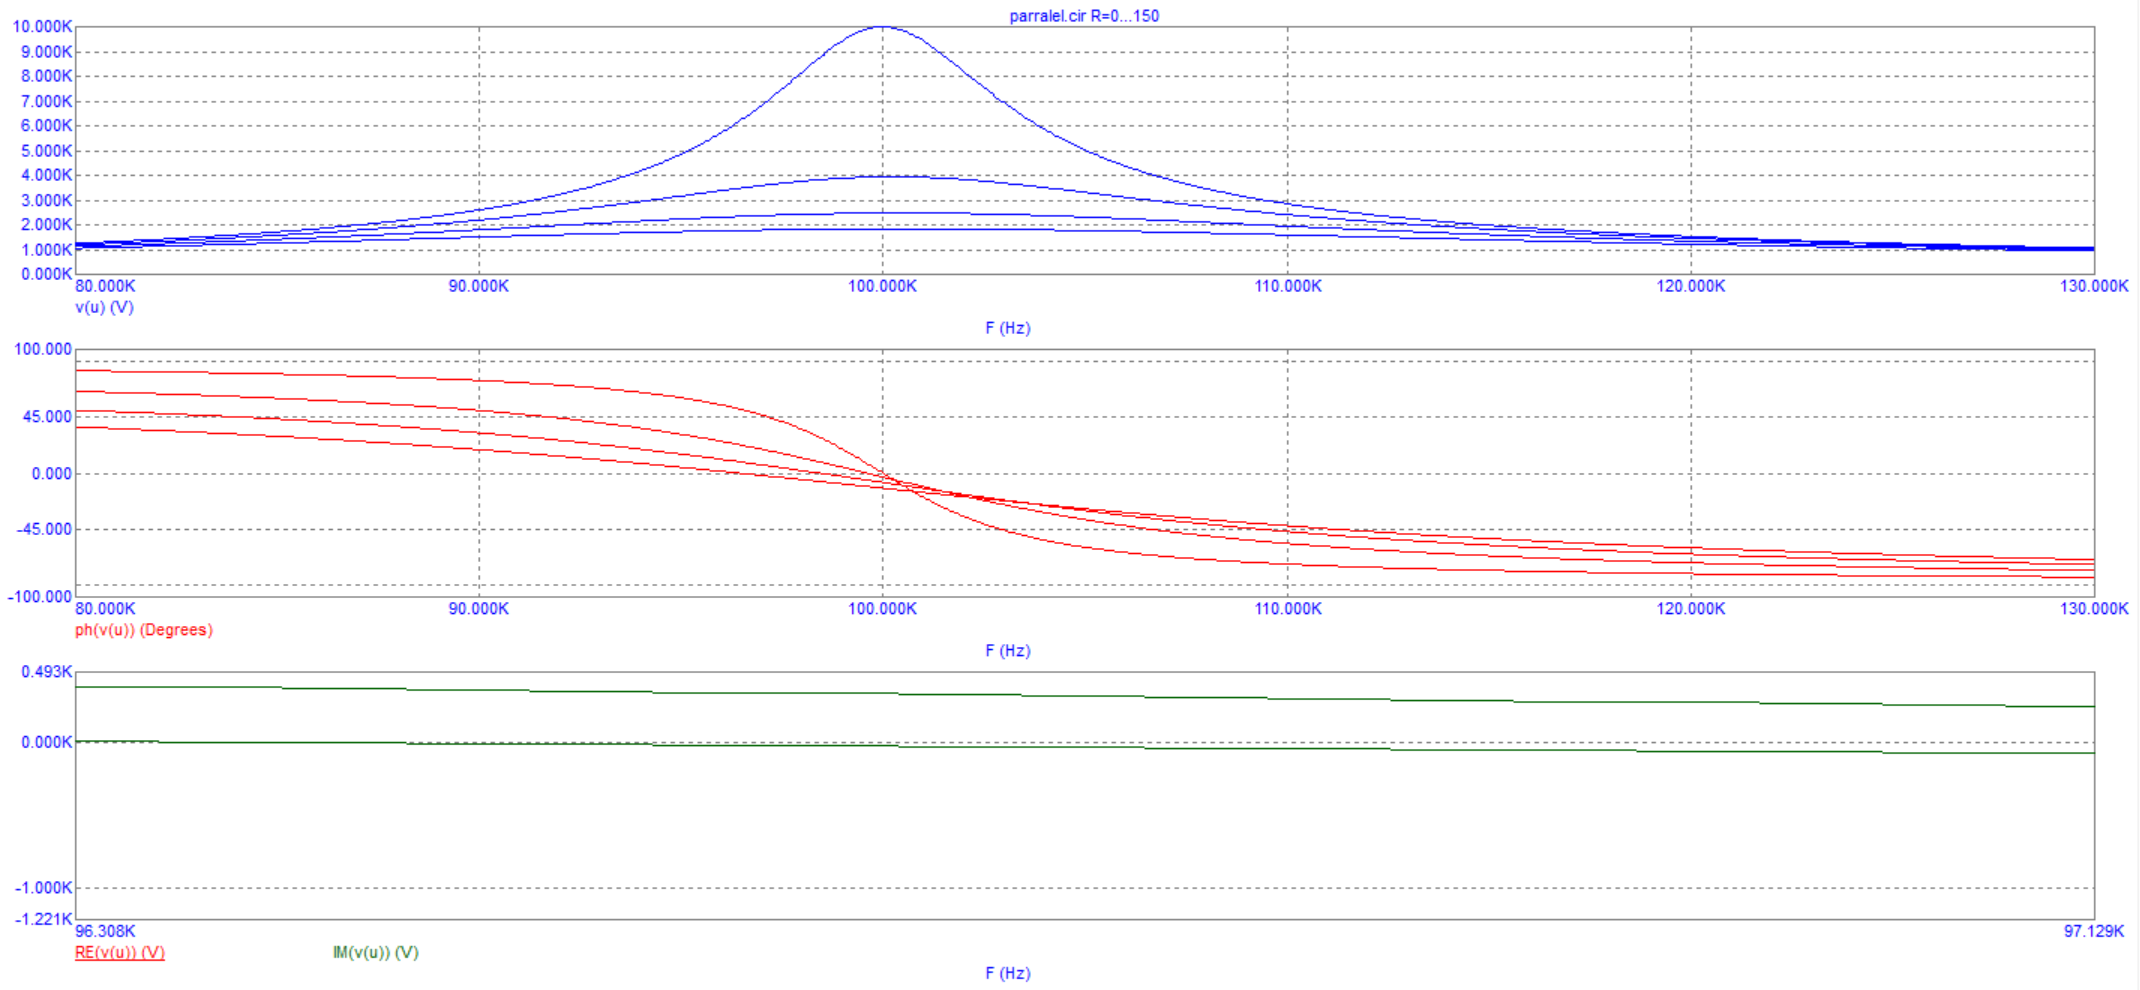
\includegraphics[scale=0.4]{parallel_AC2.png}
\label{fig:Image1}
\end{figure} 

\begin{center}
\begin{tabular}{|c|c|c|c|c|}
\hline 
$R, \: \Omega$ & 0 & 50 & 100 & 150 \\ 
\hline 
$f_{\exp}, \: kHz$ & 100 & 99,6 & 98,42 & 96,4 \\ 
\hline 
$\beta$ & 0 & 0,088 & 0,176 & 0,264 \\ 
\hline 
$f_{\exp}$ & 100 & 99,6 & 98,43 & 96,45 \\ 
\hline 
\end{tabular} 
\end{center}

\subsection{}
Исследуем влияние последовательных потерь в области низких частот. Установим частотный диапазон от $1 \: kHz$ до $130 \: kHz$ и будем варьировать $R = [0,20 \Vert 2]$.

\begin{figure}[H]
\centering
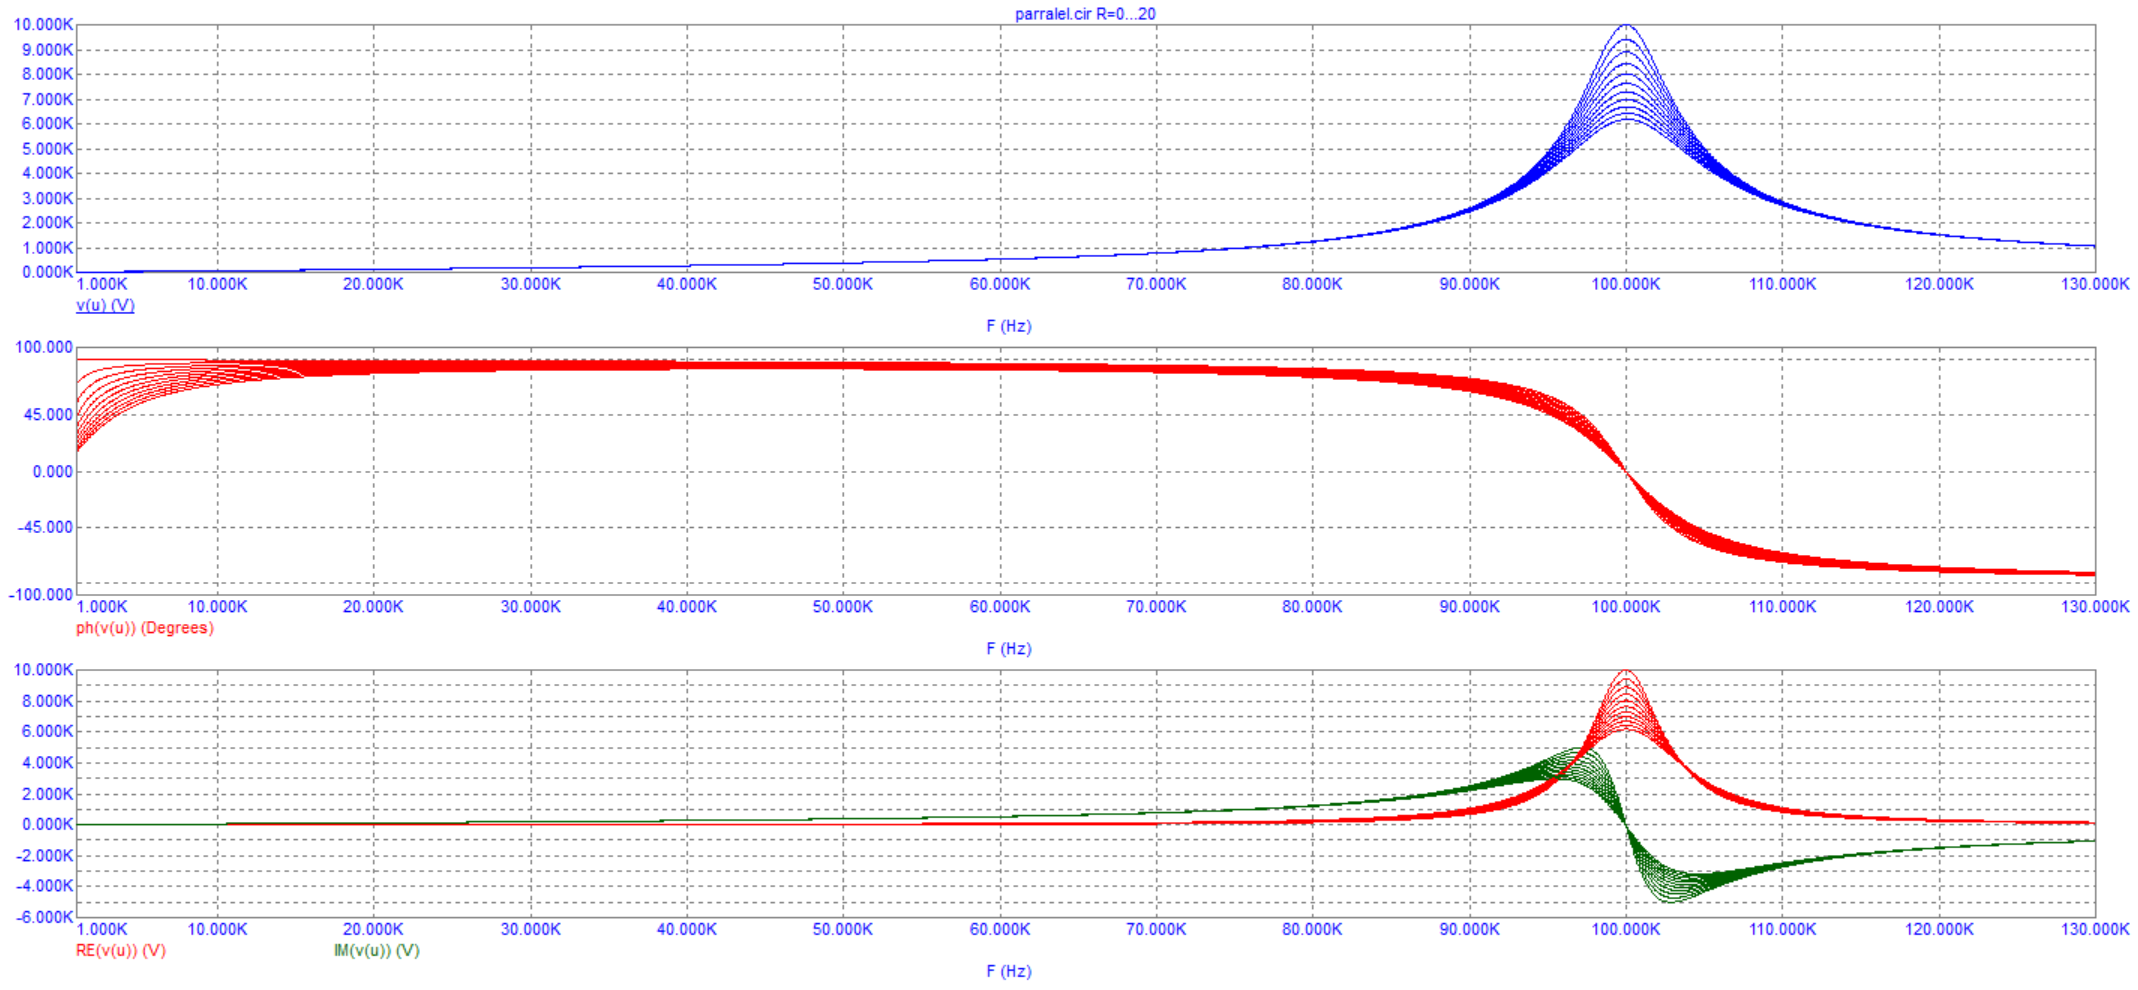
\includegraphics[scale=0.4]{parallel_AC3.png}
\label{fig:Image1}
\end{figure} 

Получаем, что при $R = 12 \: \Omega$ фазовый сдвиг на частоте $f = 2 \: kHz$ составляет $\pi / 4$. 

\section{Задание 6}

\subsection{}
Откроем модель \textbf{combined.cir} с $f_0 = 100 \: kHz$, $\rho = 15,9 \: kHz$, $q \simeq 10$, $\alpha = 1$.

\begin{figure}[H]
\centering
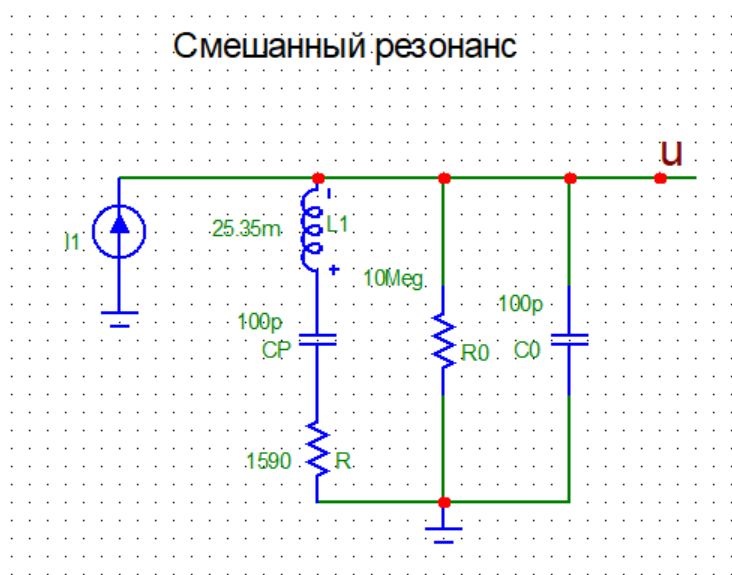
\includegraphics[scale=0.4]{combined_img.png}
\label{fig:Image1}
\end{figure}

Изучим графики частотной и фазовой характеристик, а также графики частотных зависимостей вещественной и мнимой частей мпеданса.

\begin{figure}[H]
\centering
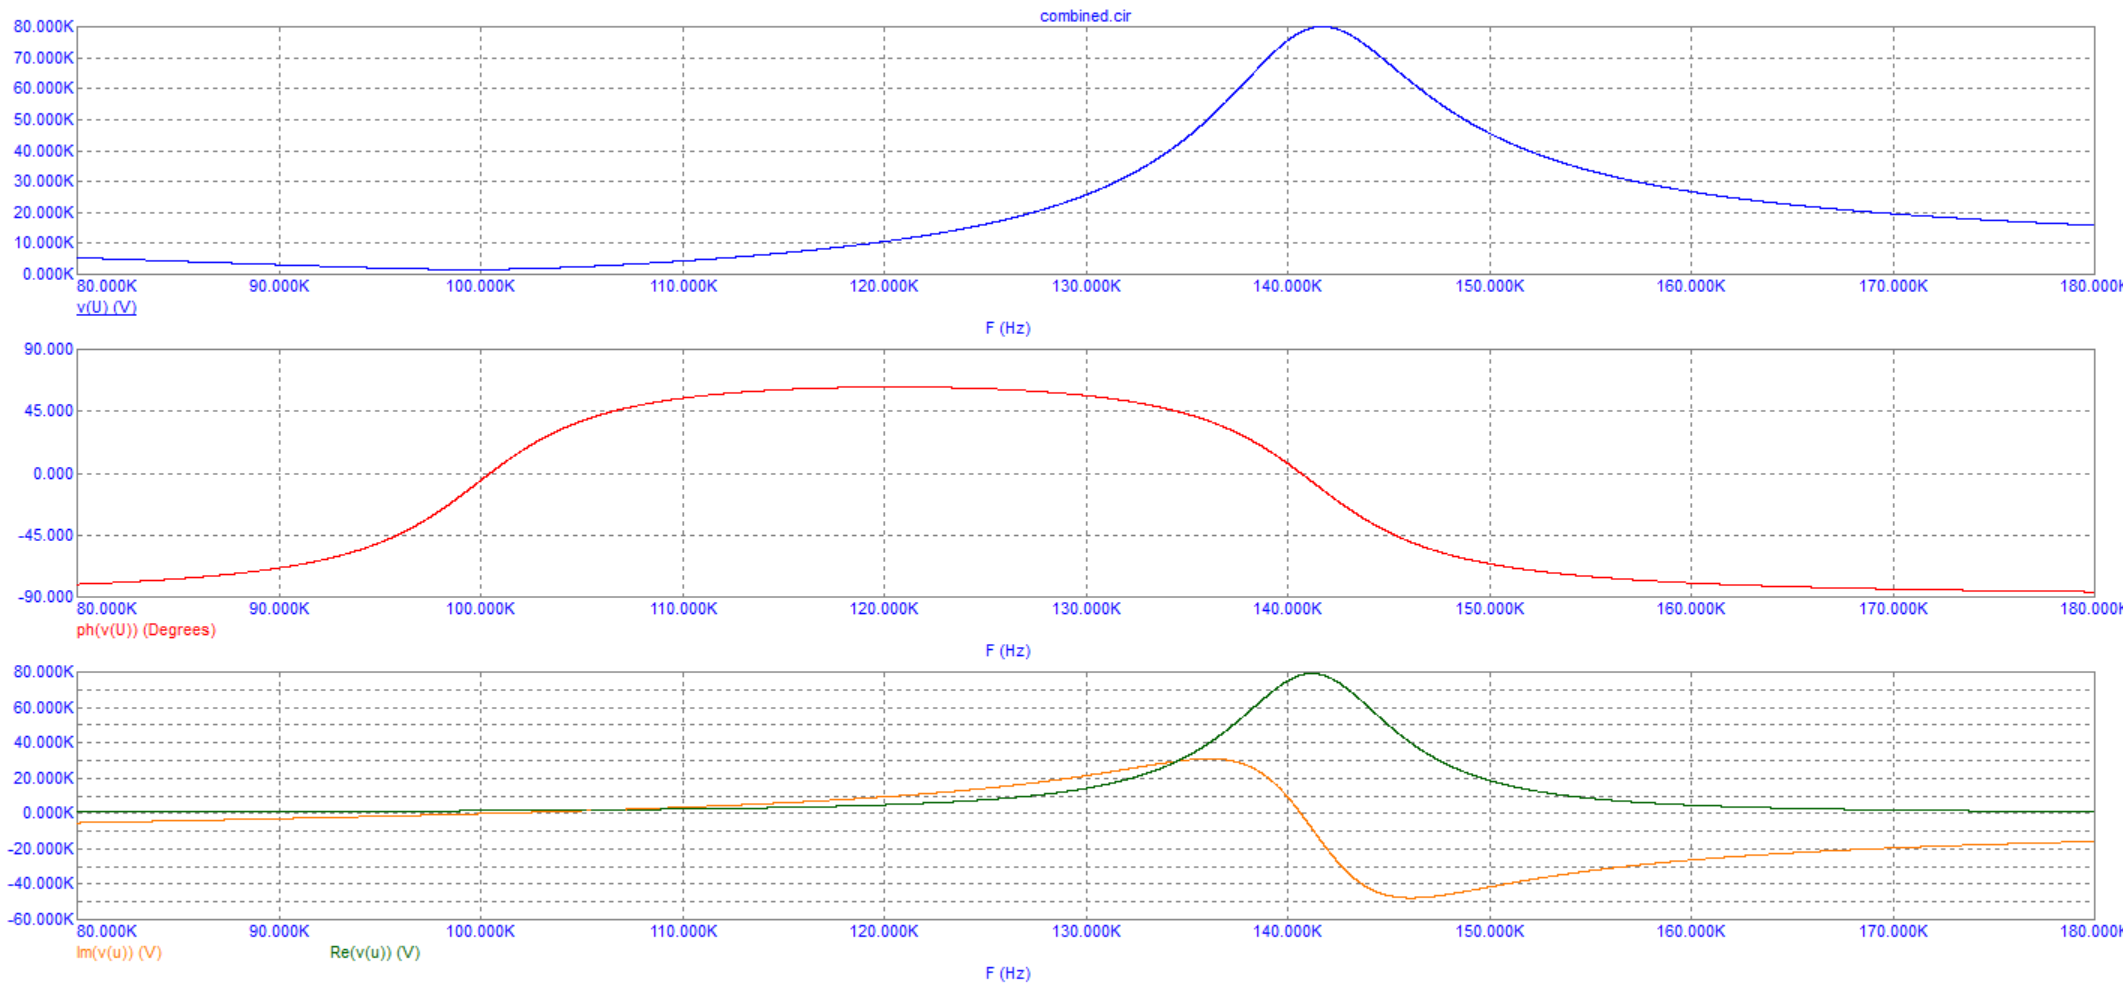
\includegraphics[scale=0.4]{combined_AC1.png}
\label{fig:Image1}
\end{figure}

\subsection{} Измерим частоты $f_p, f_0$ последовательного и параллельного резонансов по точкам пересечения нуля фазовой характеристикой:

\[f_p = 100,5 \: kHz \quad f_0 = 140,6 \: kHz\]

Измерим полосы $\triangle f_p, \triangle f_0$, в которых фазовая характеристика изменяется в диапазоне $\pm 45 \deg$ в окрестностях резонансов.

\[\triangle f_p = 10,6 \: kHz\]

\[\triangle f_0 = 10,8 \: kHz\]

Оценим добротности $Q_p, Q_0$ и проверим, что $f_0 = f_p \sqrt{2}$, $Q_0 = Q_p \sqrt{2}$:

\[Q_p = \frac{f_p}{\triangle f_p} = 9,5\]

\[Q_0 = \frac{f_0}{\triangle f_0} = 13\]

\[Q_0 = 13 \simeq 13,43 = Q_p \sqrt{2}\]

\[f_0 = 140,6 \simeq 142,1 = f_p \sqrt{2}\]

\subsection{} Измерим сопротивление контура на частотах последовательного и параллельного резонансов, сравним результаты с теоретическими значениями ($r, k^2\rho_p, Q_p$):

\[r_{exp} = 1,565 \: k\Omega \simeq 1,59 \: k\Omega = r_{\textit{th}}\]

\[(k^2\rho_p, Q_p)_{mes} = 78,1 \: k\Omega \simeq  79,1 \: k\Omega = \Big(\frac{\alpha}{1 + \alpha}\Big)^2 \sqrt{\frac{L}{c}}(1 + \alpha)\frac{r}{\rho} = (k^2\rho_p, Q_p)_{\textit{th}}\]

Снимем зависимость сопротивления на частоте параллельного резонанса от $R = [500, 2000 \Vert 500]$ и емкости $C_0 = [100p, 300p \Vert 100p]$. Сопоставим их с теорией. Осмыслим характер изменения графиков при варьировании $R$ и $C_0$.

\begin{figure}[H]
\centering
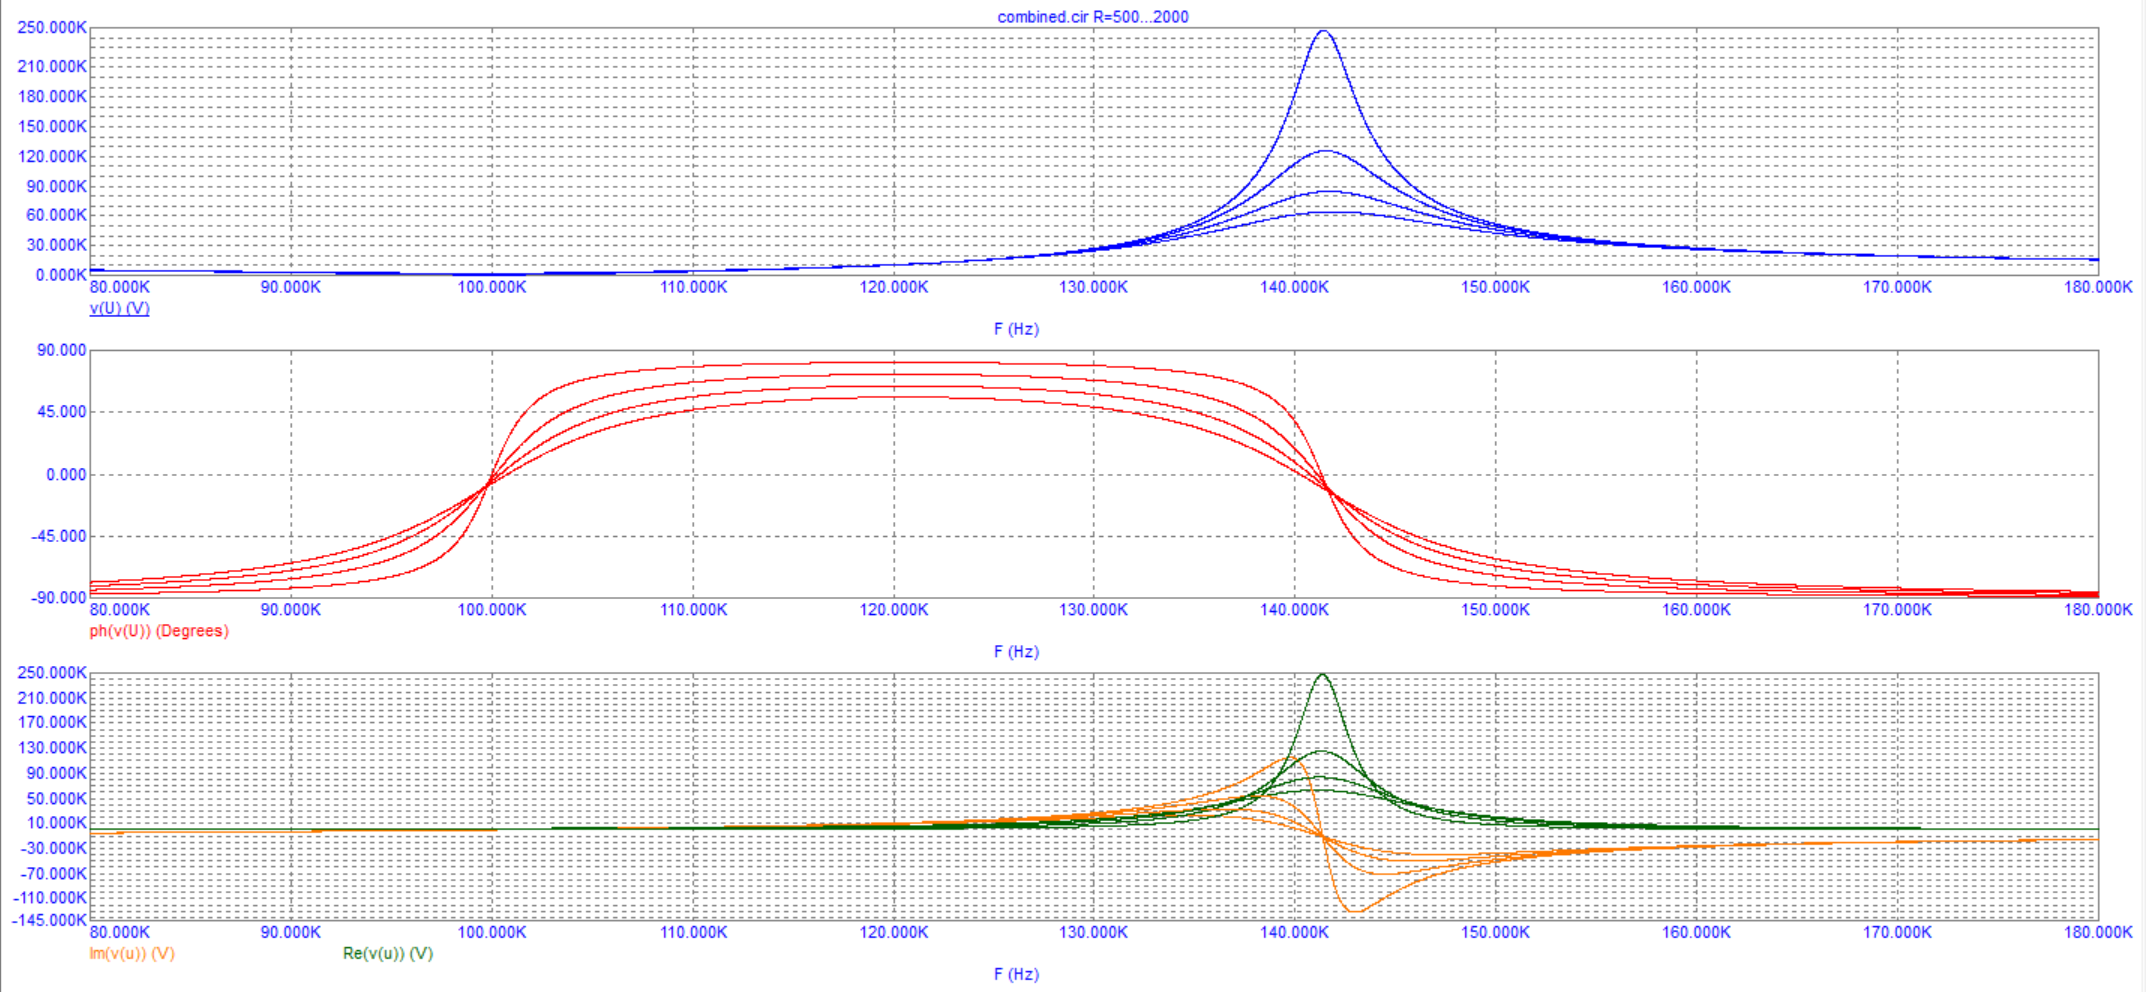
\includegraphics[scale=0.4]{combined_AC2.png}
\label{fig:Image1}
\end{figure}

\begin{center}[H]
\begin{tabular}{|c|c|c|c|c|}
\hline 
$R, \: \Omega$ & 500 & 1000 & 1500 & 2000 \\ 
\hline 
$Z, \: k\Omega$ & 247 & 124,4 & 83 & 61,9 \\ 
\hline 
\end{tabular} 
\end{center}

Получаем зависимость:

\[Z \sim \frac{1}{R}\]

\begin{figure}[H]
\centering
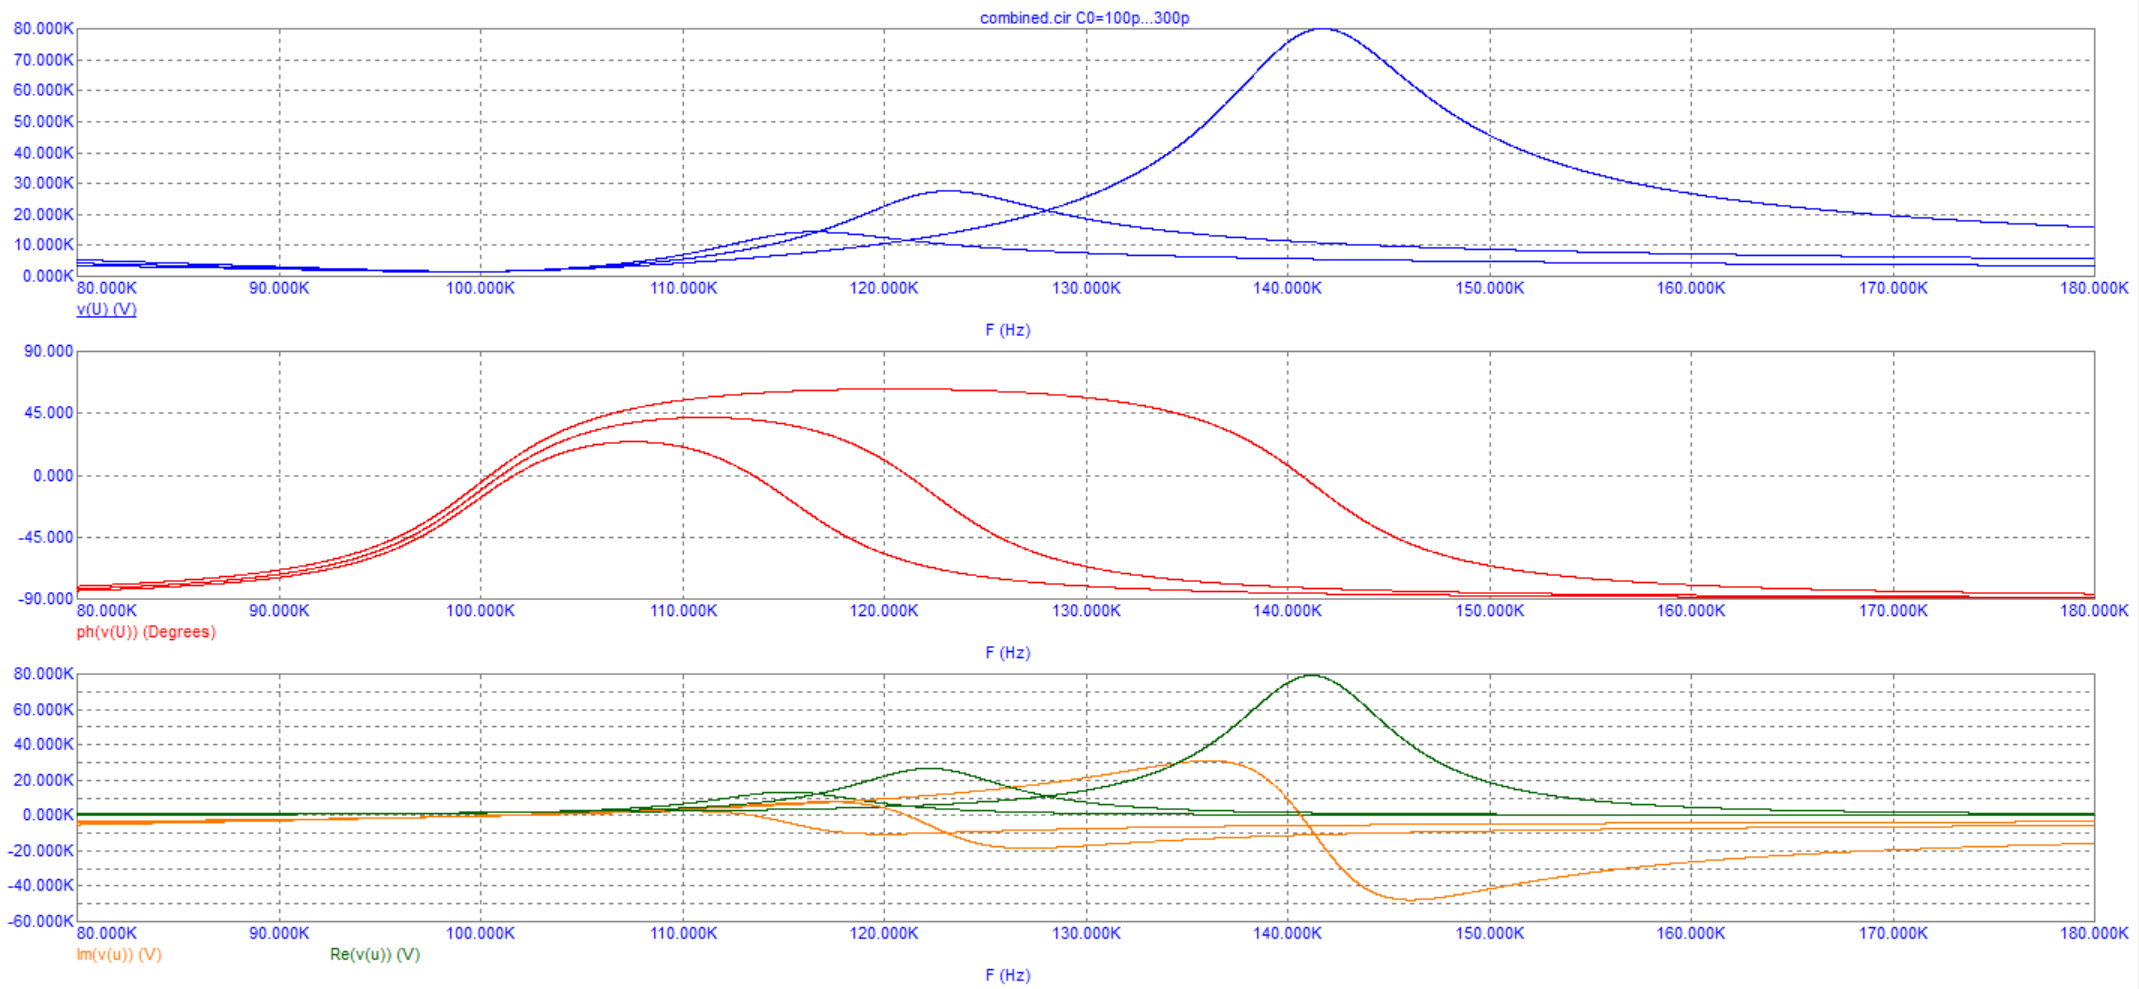
\includegraphics[scale=0.4]{combined_AC3.png}
\label{fig:Image1}
\end{figure}

\begin{center}[H]
\begin{tabular}{|c|c|c|c|}
\hline 
$C_0, \: pF$ & 100 & 200 & 300 \\ 
\hline 
$Z, \: k\Omega$ & 78,3 & 25,4 & 11,9 \\ 
\hline 
\end{tabular} 
\end{center}

Получаем зависимость:

\[Z \sim \frac{1}{C_0^2}\]

\subsection{}
Обнулим последовательности потери $r$ и варьированием $R_0 = [10k, 100k \Vert 10k]$ подберем сопротивления параллельных потерь так, чтобы достичь того же резонансного сопротивления, что и при $r = 1590 \: \Omega$.

\begin{figure}[H]
\centering
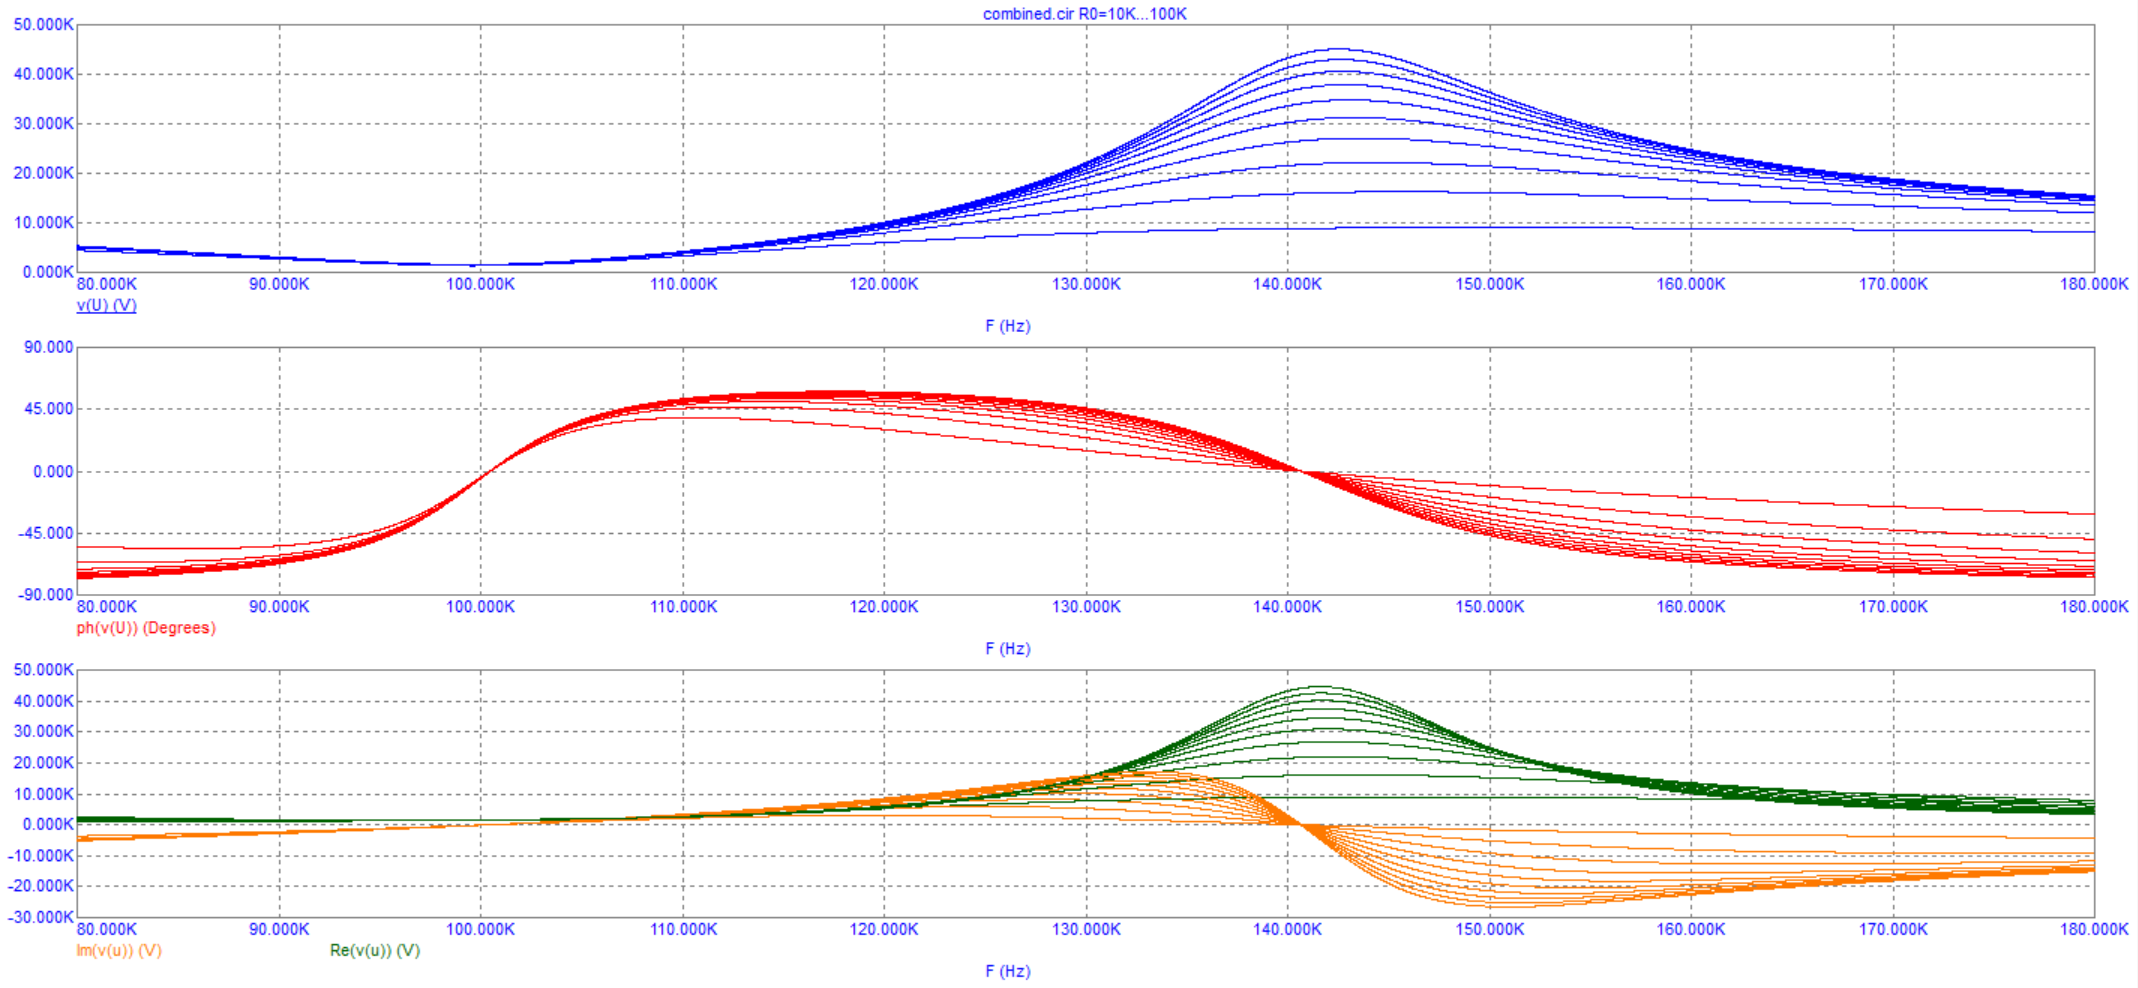
\includegraphics[scale=0.4]{combined_AC4.png}
\label{fig:Image1}
\end{figure}

Получим $R_0 = 80 \: k\Omega$. Проверим закон пересчета:

\[R_0 r = k^2 \rho_p^2\]

\[80000 \cdot 1590 \simeq \Big(\frac{1}{2}\Big)^2 \cdot 2 \cdot 15900^2.\]

Соотношение выше выполняется.

\subsection{}
Варьируя $R_0 = [80k, 10Meg \Vert 10Meg]$ при $r = 1590 \: \Omega$, изучим влияние $R_0$ на поведения частотной и фазовой характеристик на низких частотах - в диапазоне $1k, 180k$.

\begin{figure}[H]
\centering
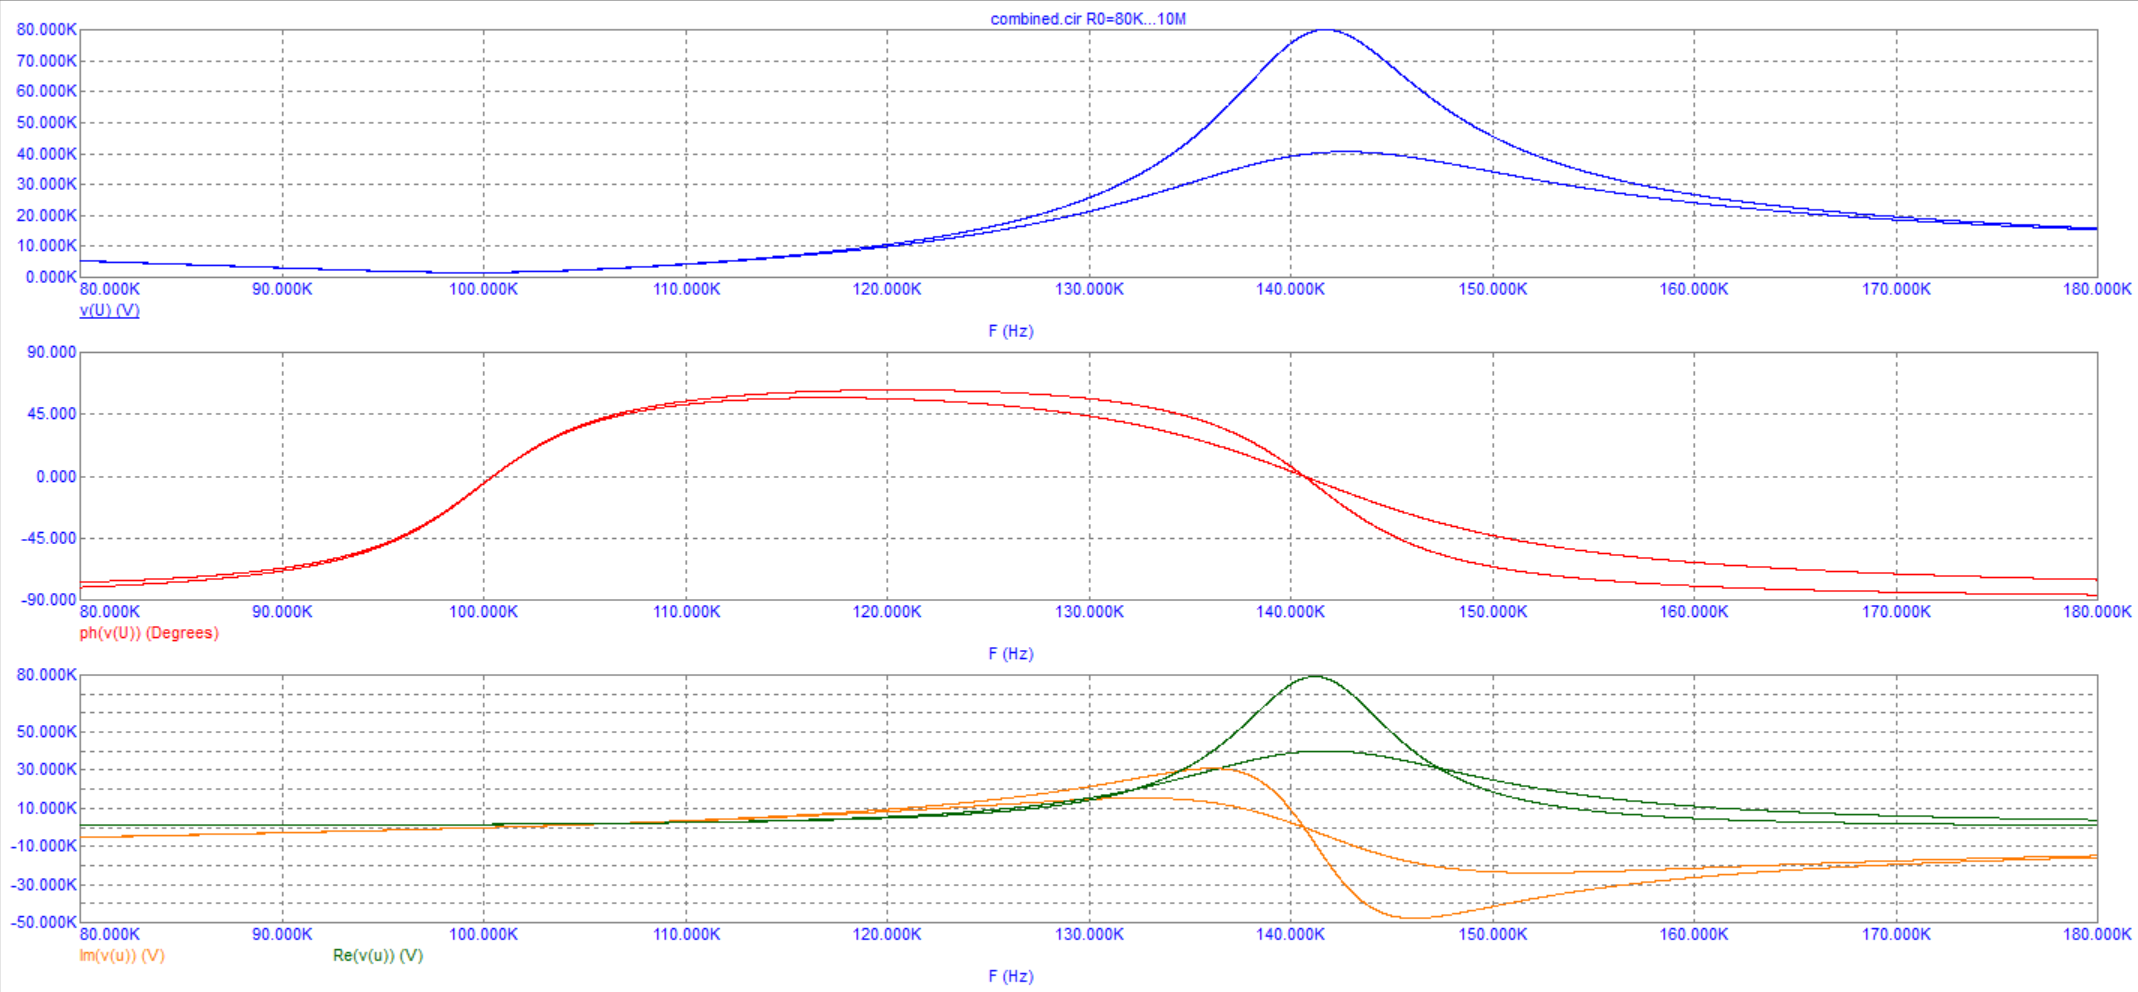
\includegraphics[scale=0.4]{combined_AC5.png}
\label{fig:Image1}
\end{figure}

При увеличении $R_0$ частотная характеристика увеличивается, а фазовая уменьшается.



\end{document}